% +------------------------------------------------------------------------+
% | CBP Reference Manual:  html_main.tex
% +------------------------------------------------------------------------+
% | Automatically generated driver file for the reference manual chapter
% | of this package used for the HTML conversion. 
% | Do not edit manually, you may loose your changes.
% +------------------------------------------------------------------------+

\input{../cebap.sty}

% +------------------------------------------------------------------------+
% | Reference manual page: Triangulation_2.tex
% +------------------------------------------------------------------------+
% | 29.03.2000   Mariette Yvinec
% | Package: Triangulation
% | 
\RCSdef{\RCSTriangulationRev}{$Revision$}
\RCSdefDate{\RCSTriangulationDate}{$Date$}
% |
%%RefPage: end of header, begin of main body
% +------------------------------------------------------------------------+

\clearpage
\section{Reference pages for Triangulation}

\subsection*{Definition}
A 
triangulation is a 2-dimensional simplicial complex which is pure
connected and without singularities. Thus a triangulation
can be viewed as a collection of triangular faces,
such that two faces either have an empty intersection or share an edge or a vertex.
The absence of singularities means that each edge belongs to 
at most two triangles and that each vertex belongs  to a set  of faces
whose union forms a topological disk.

Each face of a triangulation can be given an orientation
(clockwise or counterclockwise) which in turn induces an orientation
on the edges incident to that face. The orientation of two adjacent
faces are said to be consistent if they induce
opposite orientations on their common incident edge.
A triangulation is said to be orientable if 
the orientation of each face can be chosen in such a way
that all pairs of incident faces have consistent orientations. 

In this chapter we present a framework to represent
orientable triangulations which  may  be embedded 
in a plane or in a higher dimensional space.
Any such  triangulation can be described as a set of  vertices and
triangular faces,  with incidence and adjacence relations:
two facets or two vertices are said to be {\em adjacent}
 (or neighboring) if they are incident to the same edge,
a facet and a vertex are said to be incident if they are incident to the same
edge.

\subsection*{Design Rationale}
Because a triangulation is merely a set of
triangular faces with constant size complexity,
triangulations are not implemented
as a layer on top of a planar map.
\cgal\ uses a proper internal
representation of triangulations based on faces and vertices
rather than on edges. Such a representation
allows to save storage space and results in faster
algorithms.

Thus the basic elements of the representation are vertices and faces.
Each triangular face gives access to its three incident vertices 
and to its three adjacent faces. 
Each vertex gives access to one of its incident faces
and through that face to the circular list of its incident faces.
The edges are not explicitely represented, they are only represented 
through the adjacencies relations of two faces.


\begin{figure}
\begin{ccTexOnly}
\begin{center}
\input{three_levels.ltex}
\end{center}
\end{ccTexOnly}
\caption{The three layer design of triangulations.
\label{Triangulation_ref_Fig_three_levels}}
\begin{ccHtmlOnly}
<CENTER>
<img border=0 src=three_levels.gif align=center alt="Three_levels">
</CENTER>
\end{ccHtmlOnly}
\end{figure}



The triangulations in \cgal\ are represented
by a three layer structure  analog to the design used for polyhedral
surfaces, see Figure~\ref{Triangulation_ref_Fig_three_levels}.
In the bottom layer, the base classes for vertices and faces
store some 
geometric informations such as the coordinate of vertices 
and any other attribute (such as color, constraint edges etc.)
needed by the application.
The base classes handle
incidence and adjacency relations in term of \ccc{void*} pointers.
The use of \ccc{void*} pointers in the bottom layer allows 
to easily change one of the base
class, to deal with an extra attribute like a color for example,
without having to change the rest of the structure. 
The advantages of strong type 
checking is reestablished in the next layer 
where the \ccc{triangulation data structure} can be thought 
of as a container for faces and vertices which can take care
of all the combinatorial aspects of the triangulation.
The {triangulation data structure}
implements
adjacency and incidence relations with type safe pointer operations
and maintains the combinatorial integrity of the triangulation.
For that purpose, the {triangulation data structure} defines its own face and vertex
classes which are derived
 from the corresponding 
base classes
so that geometric and additional information on vertices and faces 
are simply inherited.
  At last, at the top layer, the \ccc{triangulation class}
implements the user interface with the triangulation. 
This classes offer to the user
the high level functionalities that can be expected from a triangulation:
insertion  or removal of a vertex, traversal of the faces,
enumeration of the vertices,
traversal of the   faces incident to a given vertex, location of a given point etc.
The {triangulation class} defines its own 
vertex and face classes
derived from the corresponding class of the {triangulation data structure}.
The vertices and faces of the {triangulation class}
are only accessed through high levels concepts such as 
handles, iterators, or circulators,
according to the required functionalities of the access.
The top layer {triangulation class}
is responsible for the geometric embedding of the triangulation
and comes in different flavors according to the kind of triangulation represented:
planar triangulation of a set of points, Delaunay or regular or constrained
 triangulations etc.

The triangulation classes of \cgal\ depends on two template parameters.
The first template parameter stands for
 a geometric traits class which is assumed to provide
the geometric objects (points, segments and triangles) 
forming  the triangulation and the geometric predicates on those objects.
The second template parameter stands for a model
of  triangulation data
structure acting as a container for faces and vertices
while  taking care of the combinatorial aspects of the triangulation. 
The triangulation data structure class is itself a template
class parametrized by the base classes for faces and vertices.


\subsection*{Concepts}
\ccRefConceptPage{Triangulation_traits_2} \\
\ccRefConceptPage{Delaunay_triangulation_traits_2} \\
\ccRefConceptPage{Regular_triangulation_traits_2} \\

\ccRefConceptPage{TriangulationDataStructure_2}\\
\ccRefConceptPage{TriangulationDataStructure_2::Face}\\
\ccRefConceptPage{TriangulationDataStructure_2::Vertex}\\
\ccRefConceptPage{TriangulationFaceBase_2}\\
\ccRefConceptPage{TriangulationVertexBase_2}\\
\ccRefConceptPage{ConstrainedTriangulationFaceBase_2}\\
\ccRefConceptPage{RegularTriangulationFaceBase_2}\\

\subsection*{Classes}
\ccRefIdfierPage{CGAL::Triangulation_2<Traits,Tds>}\\
\ccRefIdfierPage{CGAL::Delaunay_triangulation_2<Traits,Tds>}\\
\ccRefIdfierPage{CGAL::Regular_triangulation_2<Traits,Tds>}\\
\ccRefIdfierPage{CGAL::Constrained_triangulation_2<Traits,Tds>}\\
\ccRefIdfierPage{CGAL::Constrained_triangulation_demo_2<Traits,Tds>}\\
\ccRefIdfierPage{CGAL::Constrained_Delaunay_triangulation_2<Traits,Tds>}\\
\ccRefIdfierPage{CGAL::Triangulation_hierarchy_2<Tr>} \\

\ccRefIdfierPage{CGAL::Triangulation_euclidean_traits_2<R>}\\
\ccRefIdfierPage{CGAL::Triangulation_euclidean_traits_xy_3<R>}\\
\ccRefIdfierPage{CGAL::Regular_triangulation_euclidean_traits_2<Rep,Weight>}\\

\ccRefIdfierPage{CGAL::Triangulation_data_structure_using_list_2<Vb,Fb>}\\
\ccRefIdfierPage{CGAL::Triangulation_default_data_structure_2<Traits,Vb,Fb>}\\

\ccRefIdfierPage{CGAL::Triangulation_2<Traits,Tds>::Face}\\
\ccRefIdfierPage{CGAL::Triangulation_2<Traits,Tds>::Vertex}\\
\ccRefIdfierPage{CGAL::Triangulation_face_base_2<Traits>}\\
\ccRefIdfierPage{CGAL::Triangulation_vertex_base_2<Traits>}\\
\ccRefIdfierPage{CGAL::Regular_triangulation_face_base_2<Traits>}\\
\ccRefIdfierPage{CGAL::Constrained_triangulation_face_base_2<Traits>}\\

\ccRefIdfierPage{CGAL::Weighted_point<Pt,Wt>}\\
\ccRefIdfierPage{CGAL::Triangulation_cw_ccw_2}\\


\subsection*{Enum}
\ccRefIdfierPage{CGAL::Triangulation_2<Traits,Tds>::Locate_type}



% +------------------------------------------------------------------------+
%%RefPage: end of main body, begin of footer
% EOF
% +------------------------------------------------------------------------+


\begin{ccHtmlOnly}
    <HR><H2>Reference Pages</H2>
\end{ccHtmlOnly}

% +------------------------------------------------------------------------+
% | Reference manual page: Constrained_Delaunay_triangulation_2.tex
% +------------------------------------------------------------------------+
% | 12.04.2000   Author
% | Package: Package
% | 
\RCSdef{\RCSConstrainedDelaunaytriangulationRev}{$Id$}
\RCSdefDate{\RCSConstrainedDelaunaytriangulationDate}{$Date$}
% |
%%RefPage: end of header, begin of main body
% +------------------------------------------------------------------------+


\begin{ccRefClass}{Constrained_Delaunay_triangulation_2<Traits,Tds,Itag>}  %% add template arg's if necessary

%% \ccHtmlCrossLink{}     %% add further rules for cross referencing links
%% \ccHtmlIndexC[class]{} %% add further index entries

\ccDefinition
A constrained Delaunay triangulation is a triangulation with
constrained edges which tries to be as much Delaunay as possible.
Constrained edges are not necessarily Delaunay edges,
therefore a constrained Delaunay triangulation is not a Delaunay
triangulation. A constrained Delaunay is a triangulation
whose faces do not
necessarily fulfill the empty circle property
but fulfill a weaker property called the
{\em constrained empty circle}.
 To state this property,
it is convenient to think of  constrained
edges as blocking the view. Then, a triangulation is 
constrained Delaunay if
 the circumscribing circle
of any of its triangular faces includes in its interior 
no vertex  that is visible
from the interior of the triangle.  
The class \ccRefName\ is designed to represent
constrained Delaunay triangulations.

As in the case of constrained triangulations, three different versions
of Delaunay constrained triangulations are offered
depending on whether the user wishes to handle
intersecting input constraints or not.
The desired version can  be selected through the instantiation of the
third template parameter \ccc{Itag} which can be one of the
following~: \\
\ccc{CGAL::No_intersection_tag} if  intersections of
 input constraints are disallowed,\\
\ccc{CGAL::Exact_predicates_tag} allows intersections between input
constraints
 and is to be used when the traits
class
provides exact predicates but approximate constructions of the
intersection points.
\ccc{CGAL::Exact_intersections_tag} allows intersections between input
constraints
 and is to be used in conjunction
with an exact arithmetic type.


The template parameters \ccc{Tds} 
has to be instantiate with a model of \ccc{TriangulationDataStructure_2}.
The geometric traits 
of a constrained Delaunay triangulation is required
to provide the \ccc{side_of_oriented_circle} test as the geometric traits
of a Delaunay triangulation and the \ccc{Traits}
parameter has 
to be instantiated with a model
\ccc{DelaunayTriangulationTraits_2}.
When intersection of input constraints are supported, 
the geometric traits class 
is required to provide additional function object  types
to compute the intersection of two segments.
and  has then to be also a model of the concept
\ccc{ConstrainedTriangulationTraits_2}.

A constrained Delaunay triangulation is not a Delaunay
triangulation but it is a constrained triangulation.
Therefore the class \ccRefName\ derives from
the class \ccc{Constrained_triangulation_2<Traits,Tds>}.
Also, information about the status (constrained or not)
of the edges of the triangulation is stored
in the faces. 
Thus the nested \ccc{Face}
type of a constrained triangulation offers
additional functionalities to deal with this information.
These additional functionalities 
induce additional requirements on the base face class
plugged into the triangulation data structure of 
 a constrained Delaunay triangulation.
The base face of a constrained Delaunay triangulation
has to be a model of the concept
\ccc{ConstrainedTriangulationFaceBase_2}.

\cgal\ provides a default for the template parameters.
If \ccc{Gt} is the geometric traits
parameter,
the default  for
\ccc{ConstrainedTriangulationFaceBase_2}  is the class
\ccc{CGAL::Constrained_triangulation_face_base_2<Gt>}
and the default for the
triangulation data structure parameter is the class
\ccc{CGAL::Triangulation_data_structure_2<
                       CGAL::Triangulation_vertex_base_2<Gt>,
		       CGAL::Constrained_triangulation_face_base_2<Gt>
>}.
The default intersection tag is \ccc{CGAL::No_intersection_tag}.

\ccInclude{CGAL/Constrained_Delaunay_triangulation_2.h}

\ccInheritsFrom \ccc{Constrained_triangulation_2<Traits,Tds,Itag>}

\ccTypes
All types used in this class are inherited from the base class
\ccc{Constrained_triangulation_2<Traits,Tds,Itag>}.



\ccCreation
\ccCreationVariable{cdt}  %% choose variable name

\ccConstructor{Constrained_Delaunay_triangulation_2(const Traits &t = Traits())}
{Introduces an empty constrained Delaunay triangulation \ccVar.}

\ccConstructor{Constrained_Delaunay_triangulation_2(const
Constrained_Delaunay_triangulation_2& cdt1)}
 {Copy constructor, all faces and vertices
are duplicated and  the constrained status of edges
is copied.}


\ccConstructor{ template<class InputIterator> Constrained_triangulation_2(
        InputIterator first,
                               InputIterator last,
                               const Traits& t=Traits());}
{A templated constructor which introduces and builds
 a constrained triangulation with constrained edges in the range 
$\left[\right.$\ccc{first}, \ccc{last}$\left.\right)$.
\ccPrecond The \ccc{value_type} of \ccc{first} and \ccc{last}
 is \ccc{Constraint}.}



\ccHeading{Insertion and Removal}
The following member functions overwrite the corresponding
members of the base class to include a step restoring
 the Delaunay constrained
property after modification of the triangulation.

\ccMethod{ Vertex_handle insert(Point p, Face_handle f = Face_handle());}
{ Inserts point \ccc{p} in the triangulation. 
If present \ccc{f} is used as an hint
for the location of \ccc{p}.}

\ccMethod{Vertex_handle 
          insert(const Point& p,
                 Locate_type& lt,
                 Face_handle loc, int li );}
{Same as above except that the location of the point
\ccc{p}  to be inserted is assumed to be given by
\ccc{(lt,loc,i)}.}

\ccMethod{Vertex_handle push_back(const Point& p);}
{Equivalent to \ccc{insert(p)}.}

\ccMethod{template < class InputIterator >
          size_type
          insert(InputIterator first, InputIterator last);}
{Inserts the points in the range
 $\left[\right.$\ccc{first}, \ccc{last}$\left.\right)$.
 Returns the number of inserted points.
 \ccPrecond The \ccc{value_type} of \ccc{first} and \ccc{last}
 is \ccc{Point}.}

\ccMethod{ void insert_constraint(Point a, Point b);}
{ Inserts segment ab as a constrained edge in the triangulation. }

\ccMethod{ void push_back(const Constraint& c);}
{Inserts constraints \ccc{c} as above.}


\ccMethod{ void insert_constraint(Vertex_handle va, Vertex_handle vb);}
{ Inserts the line segment whose endpoints are the vertices \ccc{va} and
\ccc{vb} as a constrained  edge e in the triangulation. }


\ccMethod{void remove(Vertex_handle & v);}
{ Removes vertex v. 
\ccPrecond Vertex \ccc{v}  is not incident to a constrained edge.}

\ccMethod{ void remove_incident_constraints(Vertex_handle  v);}
{Make the edges incident to vertex \ccc{v} unconstrained edges.}

\ccMethod{void remove_constraint(const Face_handle & f, int i);}
{ Edge \ccc{(f,i)}  is no longer constrained.}


\ccHeading{Queries}
The following template member functions query the
set of faces in conflict with a point \ccc{p}.
The notion of conflict refers here to a 
constrained Delaunay setting which means the following.
Constrained edges are considered as visibility obstacles
and a point \ccc{p} is considered to be 
in conflict with a face \ccc{f} iff it is 
 visible from the interior of \ccc{f} and 
included in the circumcircle of \ccc{f}.

\ccMethod{template <class OutputItFaces, class OutputItBoundaryEdges> 
  std::pair<OutputItFaces,OutputItBoundaryEdges>
  get_conflicts_and_boundary(const Point  &p, 
			     OutputItFaces fit, 
			     OutputItBoundaryEdges eit,
                             Face_handle start) const;}
{ \ccc{OutItFaces} is an output iterator with \ccc{Face_handle} as value type.
\ccc{OutItBoundaryEdges} stands for an output iterator with \ccc{Edge} as value type.
This members function outputs in the container pointed to by \ccc{fit}
the faces which are in conflict with point \ccc{p}.
It outputs in the container pointed to by \ccc{eit} 
the boundary of the zone in conflict with \ccc{p}.
The boundary edges
of the conflict  zone are output in counterclockwise order
and each edge is described  through its incident face
which is not in conflict with \ccc{p}.
The function returns in a std::pair the resulting output iterators.
\ccPrecond dimension()==2}

\ccMethod{template <class OutputItFaces> 
	  OutputItFaces
          get_conflicts (const Point  &p, 
   		         OutputItFaces fit, 
  		         Face_handle start) const;}
{Same as above except that only the faces in conflict with \ccc{p}
are output. The function returns the resulting output iterator.
\ccPrecond dimension()==2}

\ccMethod{template <class OutputItBoundaryEdges>
          OutputItBoundaryEdges
          get_boundary_of_conflicts(const Point  &p, 
   		   		    OutputItBoundaryEdges eit,
  		       		    Face_handle start) const;}
{ \ccc{OutputItBoundaryEdges} stands for an output iterator with 
\ccc{Edge} as value
type.
 This functions  outputs in the container pointed to by \ccc{eit},
the boundary of the zone in conflict with \ccc{p}. The boundary edges
of the conflict  zone are output in counter-clockwise order
and each edge is described  through the incident face
which is not in conflict with \ccc{p}.
The function returns the resulting output iterator.}


\ccHeading{Checking}

\ccMethod{bool is_valid();}
{ Checks if the triangulation is valid and if each constrained edge is
 consistently marked constrained in its two incident faces.}

\begin{ccAdvanced}
\ccHeading{Flips}

\ccMethod{bool is_flipable(Face_handle f, int i);}
{ Determines if edge \ccc{(f,i)} can be flipped. Returns true if
edge \ccc{(f,i)} is not constrained and  the circle circumscribing f
contains  the vertex of \ccc{f->neighbor(i)}
opposite to edge \ccc{(f,i)}. }

\ccMethod{void flip(Face_handle& f, int i);}
{ Flip \ccc{f} and \ccc{f->neighbor(i)}.}


\ccMethod{void propagating_flip(List_edges & edges);}
{ Makes the triangulation constrained Delaunay by flipping edges. 
List edges contains an
initial list of edges to be flipped. The returned
triangulation is constrained Delaunay 
if the initial list contains at least all the edges of the
input triangulation that failed to be 
constrained Delaunay. (An edge is said to be 
constrained Delaunay if it is  either constrained or
locally Delaunay.) }
\end{ccAdvanced}


\ccSeeAlso
\ccc{CGAL::Constrained_triangulation_2<Traits,Tds,Itag>} \\
\ccc{TriangulationDataStructure_2} \\
\ccc{DelaunayTriangulationTraits_2} \\
\ccc{ConstrainedTriangulationTraits_2} \\
\ccc{ConstrainedDelaunayTriangulationTraits_2} \\
\ccc{ConstrainedTriangulationFaceBase_2} 

%\ccExample



%% \ccIncludeExampleCode{Package/Constrained_Delaunay_triangulation_2_prog.cpp}

\end{ccRefClass}

% +------------------------------------------------------------------------+
%%RefPage: end of main body, begin of footer
% EOF
% +------------------------------------------------------------------------+


\input{Constrained_face_base.tex}
% +------------------------------------------------------------------------+
% | Reference manual page: Constrained_triangulation_2.tex
% +------------------------------------------------------------------------+
% | 12.04.2000   Author
% | Package: Package
% | 
\RCSdef{\RCSConstrainedtriangulationRev}{$Revision$}
\RCSdefDate{\RCSConstrainedtriangulationDate}{$Date$}
% |
%%RefPage: end of header, begin of main body
% +------------------------------------------------------------------------+


\begin{ccRefClass}{Constrained_triangulation_2<Traits,Tds,Itag>}  %% add template arg's if necessary

%% \ccHtmlCrossLink{}     %% add further rules for cross referencing links
%% \ccHtmlIndexC[class]{} %% add further index entries

\ccDefinition  
A constrained triangulation is a triangulation of a set of points
which has to include among its edges 
a given set of segments joining the points. The corresponding 
edges are called {\em constrained edges}. 

The endpoints of constrained edges are of course vertices of the
triangulation. However the triangulation may include
include other vertices as well.
There are three versions of  constrained triangulations.
In the basic version, the constrained triangulation 
do not handle intersecting constraints, and the set of input 
constraints is required to be a set of segments that do not intersect
except possibly at their endpoints. Any number of constrained edges
are allowed to share the same endpoint.  Vertical constrained edges or
constrained edges with null length are allowed.
The two other versions support intersecting input constraints.
In those versions, input constraints are allowed to be
intersecting, overlapping or partially
overlapping segments.
The triangulation introduce  additional  vertices at each point which
is a proper intersection points of  two 
constraints. A single constraint intersecting other
constraints will then appear as several edges in the triangulation.
The two versions dealing with intersecting constraints, slightly differ
in the way intersecting constraints are dealt with. One of them is
designed to be robust when predicates are evaluated exactly but
constructions (i. e.  intersection computations) are
approximative.
The other one is designed to be used 
with an exact arithmetic (meaning exact
evaluation of predicates and exact computation of intersections.)
This last version finds its full efficiency  when used in conjunction
with a constraint hierarchy data structure 
as provided in the class
\ccc{Constrained_triangulation_plus_2}. See section~\ref{Section_2D_Triangulations_Constrained_Plus}.


\begin{ccTexOnly}
\begin{center} \IpeScale{50} \Ipe{constraints.ipe} \end{center}
\end{ccTexOnly}

\begin{ccHtmlOnly}
<CENTER>
<img border=0 src=constraints.gif align=center alt="A set of
constraints and its constrained triangulation">
</CENTER>
\end{ccHtmlOnly}

The class \ccRefName\ of the CGAL library
implements constrained triangulations.
The template parameter \ccc{Traits} 
stands for a geometric traits class. It has to be a model
of the concept \ccc{TriangulationTraits_2}.
When intersection of input constraints are supported, 
the geometric traits class 
is required to provide additional function object  types
to compute the intersection of two segments.
It has then to be a model of the concept
\ccc{ConstrainedTriangulationTraits_2}.
The template parameter \ccc{Tds}
stands for 
a triangulation data structure class that has to be a model
of the concept \ccc{TriangulationDataStructure_2}.
The third parameter \ccc{Itag} is the intersection tag
which serves  to choose different
strategies to deal with constraint intersections. 
\cgal\ provides three valid types for this parameter : \\
\ccc{CGAL::No_intersection_tag} disallows intersections of
 input constraints,\\
\ccc{CGAL::Exact_predicates_tag} is to be used when the traits
class
provides exact predicates but approximate constructions of the
intersection points.\\
\ccc{CGAL::Exact_intersections_tag} is to be used in conjunction
with an exact arithmetic type.

 The information about constrained edges is store in the 
faces of the triangulation. Thus the nested \ccc{Face}
type of a constrained triangulation offers
additonnal functionalities to deal with this information.
Within the design of a triangulation data structure
models templated by the base face class and the base vertex class,
these additional functionalities related to the constraints
are requirements which have to be fulfilled
by the base face.
The base face of a constrained triangulation
has to be a model of the concept
\ccc{ConstrainedTriangulationFaceBase_2}.


\cgal\ provides a defaults for the template parameters
\ccc{Tds} and \ccc{Itag}, and for the \ccc{ConstrainedTriangulationFaceBase_2}.
 If \ccc{Gt} is the geometric traits
parameter,
the default  for
\ccc{ConstrainedTriangulationFaceBase_2}  is the class
\ccc{CGAL::Constrained_triangulation_face_base_2<Gt>}
and the default for the
triangulation data structure parameter is the class
\ccc{CGAL::Triangulation_data_structure_2 <
                       CGAL::Triangulation_vertex_base_2<Gt>,
		       CGAL::Constrained_triangulation_face_base_2<Gt>
>}.
The default intersection tag is \ccc{CGAL::No_intersection_tag}.

\ccInclude{CGAL/Constrained_triangulation_2.h} 
 
\ccInheritsFrom

\ccc{Triangulation_2<Traits,Tds>}

\ccTypes
\ccTypedef{typedef pair<Point,Point> Constraint;}{ The type of input
constraints}
\ccTypedef{typedef Itag   Intersection_tag;}{The intersection tag which decides how 
intersections between input constraints are dealt with.}



\ccCreation
\ccCreationVariable{ct}  %% choose variable name

\ccConstructor{Constrained_triangulation_2();}{default constructor.}
\ccConstructor{Constrained_triangulation_2(const
Constrained_triangulation_2& ct1)}
 {Copy constructor, all faces and vertices
are duplicated and  the constrained status of edges
is copied.}

\ccConstructor{Constrained_triangulation_2(std::list<Constraint>& lc,
const Traits& t = Traits());}
{Introduces a constrained triangulation, the constrained edges of which
are the edges of the list \ccc{lc}.}

\ccConstructor{ template<class InputIterator> Constrained_triangulation_2(
        InputIterator first,
                               InputIterator last,
                               const Traits& t=Traits());}
{A templated constructor which introduces and builds
 a constrained triangulation with constrained edges in the range 
$\left[\right.$\ccc{first}, \ccc{last}$\left.\right)$.
\ccPrecond The \ccc{value_type} of \ccc{first} and \ccc{last}
 is \ccc{Constraint}.}

\ccHeading{Queries}
\ccMethod{ bool is_constrained(Edge e);}
{Returns true if edge \ccc{e} is a constrained edge.}
\ccMethod{bool are_there_incident_constraints(Vertex_handle v);}
{Returns true if at least one of the edges incident to vertex \ccc{v}
is constrained.}
\ccMethod{template<class OutputIterator>
  bool are_there_incident_constraints(Vertex_handle v, 
 OutputIterator out) const;}
{Same as above. In addition the constrained edges incident to \ccc{v}
are inserted in the sequence pointed to by the output iterator \ccc{out}.}


\ccHeading{Insertion and removal}

\ccMethod{Vertex_handle insert(Point p, Face_handle f = Face_handle() );}
{ Inserts point \ccc{p} and restores the status (constrained or not) of all
the touched edges. If present \ccc{f} is used as an hint
for the location of \ccc{p}.}

\ccMethod{Vertex_handle 
          insert(const Point& p,
                 Locate_type& lt,
                 Face_handle loc, int li );}
{Same as above except that the location of the point
 \ccc{p} to be inserted is assumed to be given by
\ccc{(lt,loc,i).}}

\ccMethod{Vertex_handle push_back(const Point& p);}
{Equivalent to \ccc{insert(p)}.}

\ccMethod{template < class InputIterator >
          int
          insert(InputIterator first, InputIterator last);}
{Inserts the points in the range
 $\left[\right.$\ccc{first}, \ccc{last}$\left.\right)$.
 Returns the number of inserted points.
 \ccPrecond The \ccc{value_type} of \ccc{first} and \ccc{last}
 is \ccc{Point}.}

\ccMethod{void insert_constraint(Point a, Point b);}
{ Inserts points a and b, and inserts segment ab as a
constraint. Removes the faces crossed by segment ab and creates new
faces instead. If a vertex c lies on segment ab, constraint ab is
replaced by the two constraints ac and cb. Apart from the insertion of
a and b, the algorithm runs in time proportionnal to the number of
removed triangles. 
\ccPrecond The relative interior of segment \ccc{ab} does not
intersect the relative interior of another constrained edge.}

\ccMethod{ void push_back(const Constraint& c);}
{Inserts constraints \ccc{c} as above.}

\ccMethod{ void insert_constraint(const Vertex_handle & va, const Vertex_handle & vb);}
{ Inserts the line segment \ccc{s} whose endpoints are the vertices 
\ccc{va} and
\ccc{vb}  as a constrained edge \ccc{e}. The triangles intersected by s
are removed and new ones are created. 
\ccPrecond The relative interior of \ccc{s} does not
intersect the relative interior of another constrained edge.  
\ccPrecond  va and vb are distinct vertices of t.  }

\ccMethod{ void insert(const Vertex_handle & va, const Vertex_handle & vb,
	    Face_handle & fr, int & i);}
{Same as above. In addition,  sets the face \ccc{fr} incident to the
egde \ccc{e} 
and on the right of \ccc{e} oriented from  \ccc{va} to \ccc{vb}
and the index \ccc{i}  of the vertex of \ccc{fr} opposite to
\ccc{e}, i.e.  \ccc{e}=\ccc{(fr,i)}.}	    

\ccMethod{void insert(const Vertex_handle & va, const Vertex_handle & vb,
	    Face_handle & fr, int & i, List_edges & new_edges );}
{Same as above. In addition,  the edges that are created are put in
the list \ccc{new\_edges}.} 

\ccMethod{void remove(const Vertex_handle & v);}
{ Removes a vertex v. 
\ccPrecond Vertex \ccc{v}  is not incident to a constrained edge.}

\ccMethod{ void remove_incident_constraints(Vertex_handle  v);}
{Make the edges incident to vertex \ccc{v} unconstrained edges.}

\ccMethod{void remove_constraint(const Face_handle & f, int i);}
{ Edge \ccc{e}=\ccc{(f,i)}=\ccc{(g,j)} is no longer constrained.}

\ccHeading{I/O}

\ccFunction{ostream & operator<<(ostream& os, const CGAL_Constrained_triangulation_2<Traits,Tds> &Ct);}
{Writes the triangulation and, for each face f, and integers i=0,1,2,
write ``C'' or ``N'' depending whether edge 
\ccc{(f,i)} is constrained or not.}

\ccSeeAlso
\ccc{CGAL::Triangulation_2<Traits,Tds>}, \\
\ccc{TriangulationDataStructure_2}, \\
\ccc{TriangulationTraits_2} \\
\ccc{ConstrainedTriangulationTraits_2} \\
\ccc{ConstrainedTriangulationFaceBase_2} \\




\ccHeading{Implementation}

%The constructors build the triangulation using a sweeping line
%algorithm. The complexity of this algorithm is $O(n\log n)$ if $n$
%endpoints are present. The sweep structure is an \stl\ map.
 The insertion of a constrained edge runs in time
proportionnal to the number of triangles intersected by this edge.

There is no need for a special implementation
of the method \ccVar\ccc{.is_valid()}
because the base class function
\ccc{ Triangulation_2<Traits>::is_valid()}
call the face class method
\ccc{Tds::Face::is_valid()} 
which, in the case of a constrained triangulation,
includes a test of the consistency of the
information about constrained edges.

\end{ccRefClass}

% +------------------------------------------------------------------------+
%%RefPage: end of main body, begin of footer
% EOF
% +------------------------------------------------------------------------+


% +------------------------------------------------------------------------+
% | Reference manual page: Constrained_triangulation_demo_2.tex
% +------------------------------------------------------------------------+
% | 13.04.2000   Author
% | Package: Package
% | 
\RCSdef{\RCSConstrainedtriangulationdemoRev}{$Revision$}
\RCSdefDate{\RCSConstrainedtriangulationdemoDate}{$Date$}
% |
%%RefPage: end of header, begin of main body
% +------------------------------------------------------------------------+


\begin{ccRefClass}{Constrained_triangulation_demo_2<Traits,Tds>}  %% add template arg's if necessary

%% \ccHtmlCrossLink{}     %% add further rules for cross referencing links
%% \ccHtmlIndexC[class]{} %% add further index entries

\ccDefinition
  
The class \ccRefName\ is intended to provide
an animation of the sweep algorithm that builds a 
constrained triangulation.

\ccInclude{Constrained_triangulation_demo_2.h}

\ccInheritsFrom
\ccc{Constrained_triangulation_2<Traits,Tds>}


\ccTypes
\ccTypedef{ typedef Window_stream Window_stream;}{}


\ccCreation
\ccCreationVariable{ctd}  %% choose variable name

\ccConstructor{Constrained_triangulation_demo_2(Window_stream& W,
                                     list<Constrained>& lc, Traits gt=Traits());}
{Outputs the created faces at each step of
the sweeping line algorithm, providing thus an animation
of the sweeping line algorithm.}


\ccSeeAlso
\ccc{CGAL::Constrained_triangulation_2<Traits,Tds>}



\end{ccRefClass}

% +------------------------------------------------------------------------+
%%RefPage: end of main body, begin of footer
% EOF
% +------------------------------------------------------------------------+


% +------------------------------------------------------------------------+
% | Reference manual page: Constrained_triangulation_face_base_2.tex
% +------------------------------------------------------------------------+
% | 12.04.2000   Author
% | Package: Package
% | 
\RCSdef{\RCSConstrainedtriangulationfacebaseRev}{$Id$}
\RCSdefDate{\RCSConstrainedtriangulationfacebaseDate}{$Date$}
% |
%%RefPage: end of header, begin of main body
% +------------------------------------------------------------------------+


\begin{ccRefClass}{Constrained_triangulation_face_base_2<Traits,Fb>}  %% add template arg's if necessary

%% \ccHtmlCrossLink{}     %% add further rules for cross referencing links
%% \ccHtmlIndexC[class]{} %% add further index entries
\ccCreationVariable{ctfb} 

\ccDefinition
 The class \ccRefName\ is the default model for the concept
\ccc{ConstrainedTriangulationFaceBase_2} to be used as base face class
of constrained triangulations.

\ccInclude{CGAL/Constrained_triangulation_face_base_2.h}

\ccIsModel
\ccc{ConstrainedTriangulationFaceBase_2}

\ccParameters
The first template parameter is a geometric traits.

The second template parameter has to be a model
of the concept \ccc{TriangulationFaceBase_2}.
Its default is \ccc{CGAL::Triangulation_face_base_2<Traits>}

\ccInheritsFrom
The class \ccRefName\  derives from its parameter \ccc{Fb}.
and add three Boolean to deal with information about
constrained edges.

The member functions \ccc{cw(int i)}, \ccc{ccw(int i)}
and \ccc{reorient} are overloaded  to update
information about constrained edges.

\ccSeeAlso
\ccc{TriangulationFaceBase_2} \\
\ccc{ConstrainedTriangulationFaceBase_2}\\
\ccc{CGAL::Constrained_triangulation_2<Traits,Tds>} \\
\ccc{CGAL::Triangulation_face_base_2<Traits>}


\end{ccRefClass}

% +------------------------------------------------------------------------+
%%RefPage: end of main body, begin of footer
% EOF
% +------------------------------------------------------------------------+


% +------------------------------------------------------------------------+
% | Reference manual page: Delaunay_triangulation_3.tex
% +------------------------------------------------------------------------+
% | 20.03.2005   Author Daniel Russel
% | Package: Kinetic_data_structures
% | 
\RCSdef{\RCSDelaunaytriangulationRev}{$Id$}
\RCSdefDate{\RCSDelaunaytriangulationDate}{$Date$}
% |
%%RefPage: end of header, begin of main body
% +------------------------------------------------------------------------+


\begin{ccRefClass}{Kinetic::Delaunay_triangulation_2<Traits, Visitor, Triangulation>}  %% add template arg's if necessary

%% \ccHtmlCrossLink{}     %% add further rules for cross referencing links
%% \ccHtmlIndexC[class]{} %% add further index entries

\ccDefinition
  
The class \ccRefName\ maintains a Delaunay triangulation on top of the
points contained in a \ccc{Kinetic::ActiveObjectsTable}. It has one main method
of interest. \ccc{triangulation()} which returns the triangulation it
is maintaining. 

The class \ccc{Kinetic::Qt_triangulation_2<KineticTriangulation_2,
QtWidget_2, QtMovingPoints_2>} displays a kinetic Delaunay
triangulation using the Qt widget.

This class is a good example of a simple, but non-trivial, kinetic
data structure.

The Triangulation template parameter must use
\ccc{Traits::Instantaneous_kernel} as its geometric traits and the
\ccc{Triangulation::Face} must inherit from \ccc{Kinetic::Delaunay_triangulation_face_base_2<Traits, Base>}.

The optional \ccc{Visitor} parameter takes a model of
Kinetic::DelaunayTriangulationVisitor2. Methods on this object will be called
whenever the triangulation changes.

\ccInclude{CGAL/Kinetic/Delaunay_triangulation_2.h}

\ccIsModel

\ccc{Ref_counted<T>}


\ccTypes

\ccNestedType{Triangulation}{The type of the Delaunay triangulation it maintains. This is a \ccc{CGAL::Delaunay_triangulation<Traits, Tds>} built using the \ccc{Kinetic::InstantaneousKernel} as the kernel.}

\ccCreation
\ccCreationVariable{dt}  %% choose variable name

\ccConstructor{Delaunay_triangulation_2(Traits tr);}{Maintain the Delaunay triangulation of the points in \ccc{mot}.}

\ccOperations

\ccMethod{const Triangulation& triangulation();}{Access the triangulation that is maintained. }

\ccSeeAlso

Kinetic::DelaunayTriangulationVisitor2,
\ccc{Kinetic::Delaunay_triangulation_default_visitor_2},
\ccc{Kinetic::Delaunay_triangulation_recent_edges_visitor_2<Triangulation>},
\ccc{Kinetic::Delaunay_triangulation_event_log_visitor_2},
\ccc{Kinetic::Qt_Delaunay_triangulation_2}.


\end{ccRefClass}

% +------------------------------------------------------------------------+
%%RefPage: end of main body, begin of footer
% EOF
% +------------------------------------------------------------------------+


% +------------------------------------------------------------------------+
% | Reference manual page: Delaunay_triangulation_traits_2.tex
% +------------------------------------------------------------------------+
% | 12.04.2000   Author
% | Package: Package
% | 
\RCSdef{\RCSDelaunaytriangulationtraitsRev}{$Revision$}
\RCSdefDate{\RCSDelaunaytriangulationtraitsDate}{$Date$}
% |
%%RefPage: end of header, begin of main body
% +------------------------------------------------------------------------+


\begin{ccRefConcept}{Delaunay_triangulation_traits_2}

%% \ccHtmlCrossLink{}     %% add further rules for cross referencing links
%% \ccHtmlIndexC[concept]{} %% add further index entries

\ccDefinition
  
The concept \ccRefName\ does this and that.
In addition to the requirements 
of the concept \ccc{Triangulation_traits_2}
described \ccRefPage{Triangulation_traits_2},
the concept \ccRefName\
has to  provide a \ccc{side_of_oriented_circle} test
and some additional types.
The \ccc{side_of_oriented_circle} test is the test used to maintain the
empty circle property and actually defines the triangulation.
The additional types \ccc{Line}, \ccc{Direction}
and \ccc{Ray} are used to describe the dual Voronoi diagram.
The additional \ccc{Distance} type is only used by the
\ccc{nearest_vertex(..)} query and the requirements for this type
are given below.


\ccTypes
\ccNestedType{Line}
\ccGlue
\ccNestedType{Ray}{}
\ccGlue
\ccNestedType{Direction}{}
\ccNestedType{Distance}{Needed only if the \ccc{nearest_neighbor()} 
function is called.}

Each of the three classes \ccc{Line}, \ccc{Direction} and 
\ccc{Ray}  must know the two others.
In addition, the \ccc{Line} class is required to have the two
following member functions:
\begin{ccClass}{Line}

\ccCreationVariable{l}
\ccThree{Direction }{l.direction()x}{}
\ccMethod{Line opposite();}{the same line with opposite orientation.}
\ccGlue
\ccMethod{Direction direction();}{the direction of the line.}
\end{ccClass}
The \ccc{Ray} class must define a \ccc{Point} class which is the same
as \ccc{Traits::Point} 
is required to have the following constructor:

\begin{ccClass}{Ray}
\ccCreationVariable{r}
\ccConstructor{Ray(Traits::Point p, Direction d);}{}
\end{ccClass}


\ccCreation
\ccCreationVariable{traits}  %% choose variable name

\ccConstructor{Delaunay_triangulation_traits_2();}{default constructor.}

\ccPredicates
\ccMethod{Oriented_side side_of_oriented_circle(const Point& p0,
                                                     const Point& p1,
                                                     const Point& p2,
                                                     const Point& test);}
{Gives the \ccc{Oriented_side} of point \ccc{test} with respect to
the oriented circumscribing circle of  points \ccc{p0, p1} and \ccc{p2}.
This answers the \ccc{in_circle}  test if the \ccc{Orientation}
of  Points \ccc{p0, p1} and \ccc{p2} is known,
which is the case for the points associated with the three
vertices of a triangulation face.}


\ccOperations
\ccMethod{Point circumcenter(const Point &p, const Point &q, const
Point &r) const;} { Returns the center point equidistant from \ccc{p}, \ccc{q} and
\ccc{r}. This method is required only if the duality functions are called.}

\ccMethod{Line bisector(const Segment &s);}
{Returns the bisector line of segment s. This method is required only if duality functions
are called.}

\ccHasModels
\ccc{CGAL::Triangulation_euclidean_traits_2<Rep>},
\ccc{CGAL::Triangulation_euclidean_traits_xy_3<Rep>},
\ccc{CGAL::Triangulation_euclidean_traits_yz_3<Rep>},
\ccc{CGAL::Triangulation_euclidean_traits_zx_3<Rep>}.


\end{ccRefConcept}

% +------------------------------------------------------------------------+
%%RefPage: end of main body, begin of footer
% EOF
% +------------------------------------------------------------------------+


% +------------------------------------------------------------------------+
% | Reference manual page: Locate_type.tex
% +------------------------------------------------------------------------+
% | 06.04.2000   Author
% | Package: Package
% | 
\RCSdef{\RCSLocatetypeRev}{$Revision$}
\RCSdefDate{\RCSLocatetypeDate}{$Date$}
% |
%%RefPage: end of header, begin of main body
% +------------------------------------------------------------------------+

\ccModifierCrossRefOff
\begin{ccRefEnum}[Triangulation_2<Traits,Tds>::]{Locate_type}  %% add template arg's if necessary

%% \ccHtmlCrossLink{}     %% add further rules for cross referencing links
%% \ccHtmlIndexC[enum]{} %% add further index entries

\ccDefinition
  
The enum \ccRefName\ is defined by the
\ccc{Triangulation_2<Traits,Tds>} 
class to specify
which case occurs when locating a point in the triangulation. 

\ccEnum{enum Locate_type {VERTEX=0, EDGE, FACET, OUTSIDE_CONVEX_HULL, 
OUTSIDE_AFFINE_HULL};}
{The locate type is :
\ccc{VERTEX} when the located point coincides 
with a vertex of the triangulation \\
\ccc{EDGE} when it is located on the relative interior of an edge \\
\ccc{FACE} when it is located on the interior of a face  \\
\ccc{OUTSIDE_CONVEX_HULL} when the point
is  outside the convex hull but in the affine hull of the current triangulation \\
\ccc{OUTSIDE_AFFINE_HULL} 
when the point is outside the affine hull
of the current triangulation.}

\ccSeeAlso
\ccc{CGAL::Triangulation_2<Traits,Tds>}.

\end{ccRefEnum}
\ccModifierCrossRefOn



% +------------------------------------------------------------------------+
%%RefPage: end of main body, begin of footer
% EOF
% +------------------------------------------------------------------------+


\input{Regular_face_base.tex}
% +------------------------------------------------------------------------+
% | Reference manual page: Regular_triangulation_traits_2.tex
% +------------------------------------------------------------------------+
% | 12.04.2000   Author
% | Package: Package
% | 
\RCSdef{\RCSRegulartriangulationtraitsRev}{$Revision$}
\RCSdefDate{\RCSRegulartriangulationtraitsDate}{$Date$}
% |
%%RefPage: end of header, begin of main body
% +------------------------------------------------------------------------+


\begin{ccRefConcept}{Regular_triangulation_traits_2}

%% \ccHtmlCrossLink{}     %% add further rules for cross referencing links
%% \ccHtmlIndexC[concept]{} %% add further index entries

\ccDefinition
  
The concept \ccRefName\ fulfill the requirements of
concept \ccc{Triangulation_traits_2} 
described \ccRefPage{Triangulation_traits_2}
and additionally provides  a type
\ccc{Weitghed_point}  (which derives from the type \ccc{Point} 
and add a weight data member )
and the power tests for weighted points.
The traits must also provide the types 
\ccc{Ray} and \ccc{Line} to output the dual power diagram,
and also eventually a \ccc{Distance} type 
(analogue to the distance type defined in concept
\ccc{Delaunay_triangulation_traits_2}
to answer to lowest power query (localisation in the power diagram).


\ccTypes
\ccNestedType{Bare_point}
\ccGlue    
\ccNestedType{Weighted_point}
\ccGlue
\ccNestedType{Line}{}
\ccGlue
\ccNestedType{Ray}{}
\ccGlue
\ccNestedType{Direction}{}
\ccGlue
\ccNestedType{Distance} {NOT YET required.}
 

\ccCreation
\ccCreationVariable{traits}  %% choose variable name

\ccConstructor{Regular_triangulation_traits_2();}{default constructor.}

\ccPredicates
\ccMethod
{Oriented_side  power_test(const Weighted_point &p,
                           const Weighted_point &q,
                           const Weighted_point &r,
                           const Weighted_point &s);} 
{The two dimensional  power test.}
\ccMethod
{Oriented_side  power_test(const Weighted_point &p,
                           const Weighted_point &q,
                           const Weighted_point &r);}
{The degenerate one dimensional power test  for collinear
Weighted points.
\ccPrecond The points included in \ccc{p}, \ccc{q} 
and \ccc{r} are collinear.}

\ccOperations
\ccMethod{Rt power(Weighted_point wp, Weighted_point wq) const;}{Returns the power product
of \ccc{wp} \ and \ccc{wq}. This function is NOT YET required nor used.}


\ccHasModels

\ccc{CGAL::Regular_triangulation_traits_2<Rep>}


\end{ccRefConcept}

% +------------------------------------------------------------------------+
%%RefPage: end of main body, begin of footer
% EOF
% +------------------------------------------------------------------------+


% +------------------------------------------------------------------------+
% | Reference manual page: Regular_triangulation_2.tex
% +------------------------------------------------------------------------+
% | 12.04.2000   Author
% | Package: Package
% | 
\RCSdef{\RCSRegulartriangulationRev}{$Revision$}
\RCSdefDate{\RCSRegulartriangulationDate}{$Date$}
% |
%%RefPage: end of header, begin of main body
% +------------------------------------------------------------------------+


\begin{ccRefClass}{Regular_triangulation_2<Traits,Tds>}  %% add template arg's if necessary

%% \ccHtmlCrossLink{}     %% add further rules for cross referencing links
%% \ccHtmlIndexC[class]{} %% add further index entries

\ccDefinition
  
The class \ccRefName\ 
is designed to maintain the
regular triangulation of a set of weighted points.


Let ${  PW} = \{(p_i, w_i), i = 1, \ldots , n \}$ be a set of 
weighted points where each $p_i$ is a point and each $w_i$
is a scalar called the weight of point $p_i$.
Alternatively, each weighted point $(p_i, w_i)$ can be regarded
as a two dimensional sphere with center $p_i$ and radius $r_i=\sqrt{w_i}$.

The power diagram of the set ${  PW}$ is a planar partition 
such that each cell corresponds to sphere $(p_i, w_i)$ of ${  PW}$
and is the locus of points  $p$ whose power with respect to $(p_i, w_i)$
is less than its power with respect to any other sphere $(p_j, w_j)$
in ${  PW}$. 
The dual of this diagram is a triangulation 
whose domain covers the convex hull of the set 
${  P}= \{ p_i, i = 1, \ldots , n \}$ of center points
and whose vertices are a subset of ${  P}$.
Such a triangulation is called a regular triangulation.
The  three points $p_i, p_j$ and $p_k$ of ${  P}$
form a triangle in the regular triangulation of ${  PW}$
iff there is a point $p$ of the plane whose
powers with respect to $(p_i, w_i)$, $(p_j, w_j)$
and $(p_k, w_k)$ are equal and less than the power of $p$
with respect to any other sphere in  ${  PW}$.

Let us defined the power product of two weighted points
$(p_i, w_i)$ and $(p_j, w_j)$ as:
\[\Pi(p_i, w_i,p_j, w_j) = p_ip_j ^2 - w_i  - w_j  .\]
$\Pi(p_i, w_i,p_j, 0)$ is simply the power of point $p_j$
with respect to the sphere $(p_i, w_i)$, and two weighted points 
are said to be orthogonal if their power product is null.
The power circle of three weighted points
 $(p_i, w_i)$, $(p_j, w_j)$
and $(p_k, w_k)$ is defined as the unique circle
$(\pi, \omega)$  orthogonal to
 $(p_i, w_i)$, $(p_j, w_j)$
and $(p_k, w_k)$.

The regular triangulation of the sets ${  PW}$
satisfies the following {\em regular property} (which just reduces to the 
Delaunay property when all the weights are null):
a triangle $p_ip_jp_k$ of the regular triangulation
of ${  PW}$ is such that the power product of any weighted point
 $(p_l, w_l)$ of ${  PW}$ with the power circle of
 $(p_i, w_i)$, $(p_j, w_j)$ is $(p_k, w_k)$ is positive or null.
We call  power test of the weighted point $(p_l, w_l)$ with respect
to the face  $p_ip_jp_k$, the predicates which amount to compute
the sign of 
the power product of $(p_l, w_l)$ with respect to
the power circle of
 $(p_i, w_i)$, $(p_j, w_j)$ is $(p_k, w_k)$,
which is given by the following
determinant
\[\left| \begin{array}{cccc}
1  &  x_i  &  y_i  &  x_i ^2 + y_i ^2 - w_i  \\
1  &  x_j  &  y_j  &  x_j ^2 + y_j ^2 - w_j  \\
1  &  x_k  &  y_k  &  x_k ^2 + y_k ^2 - w_k  \\
1  &  x_l  &  y_l  &  x_l ^2 + y_l ^2 - w_l
\end{array}
\right|
\]

A pair of neighboring faces $p_ip_jp_k$
and $p_ip_jp_l$ is said to be locally regular
(with respect to  the weights in ${  PW}$)
if the power test of $(p_l,w_l)$ with respect to
$p_ip_jp_k$ is positive.
A classical  result of computational geometry
establishes that a triangulation of the convex hull of ${  P}$
such that any pair of neighboring faces is regular with respect
to ${  PW}$, is a
 regular triangulation of ${  PW}$.

Alternatively, the regular triangulation
of the weighted points set ${  PW}$
can be obtained as the projection
on the two dimensional plane of the convex hull of the set of three
dimensional points 
${  P'}= \{ (p_i,p_i ^2 - w_i ), i = 1, \ldots , n \}$.



 
A Regular triangulation is a special triangulation of a set of points,
so it is natural to derive  the class \ccRefName\
from the basic class \ccc{Triangulation_2<Traits,Tds>}.
The template parameters \ccc{Traits} and \ccc{Tds} 
are to be instantiated with models of respectively
\ccc{RegularTriangulationTraits_2}  and
\ccc{TriangulationDataStructure_2}.


The concept of triangulation data structure
is described in \ccRefPage{TriangulationDataStructure_2}
and the same models can be used to instantiate the
triangulation data structure of either a \ccc{Triangulation_2<Traits,Tds>}
or a \ccRefName.
The  concept of \ccc{RegularTriangulationTraits_2},
described page~\ccRefPage{RegularTriangulationTraits_2}, 
must provide a weighted point type
and a power test on these weighted points. 

\ccInclude{Regular_triangulation_2.h}

\ccInheritsFrom
\ccc{Triangulation_2<Traits,Tds>}

\ccTypes
\ccThree{typedef Traits::Weighted_point}{Weighted_point;}{}
\ccThreeToTwo
\ccTypedef{typedef Traits::Distance Distance;}{}

\ccTypedef{typedef Traits::Line Line;}{}
\ccGlue
\ccTypedef{typedef Traits::Direction Direction;}{}
\ccGlue
\ccTypedef{typedef Traits::Ray Ray;}{}
\ccGlue
\ccTypedef{typedef Traits::Bare_point  Bare_point;}{}
\ccGlue
\ccTypedef{typedef Traits::Weighted_point  Weighted_point;}{}


\ccCreation
\ccCreationVariable{rt}  %% choose variable name

\ccConstructor{Regular_triangulation_2(const Traits& gt = Traits());}
{Introduces an empty regular triangulation \ccVar.}

\ccConstructor{Regular_triangulation_2(const Regular_triangulation_2 &rt);}
{Copy constructor.}


\ccHeading{Insertion and Removal}

The vertices of the regular triangulation
of a set of weighted points ${  PW}$ form only a subset
of the set of center points of ${   PW}$.
Therefore the  insertion of a weighted point  in a regular triangulation
does not necessarily imply the creation of a new vertex.
If the new inserted point does not appear as a vertex in the
regular triangulation, it is said to be hidden 
by the face in which the corresponding center point is located.
Such a weighted point is stored in a list attached to the hiding face,
to be used for later tentative of insertions when future removal
of some points implies the destruction of the hiding face.


\ccThree{Vertex_handle}{T.push_back(const Point &p);}{}

\ccMethod{bool insert(const Weighted_point& p, Face_handle f=Face_handle());}
{inserts  weighted point \ccc{p} and 
returns true if a new vertex is created. 
If a weighted point with the same center point but a 
different weight already exists in the triangulation, 
it is removed and replaced by the new point.
If given the parameter \ccc{f} is used as an hint
for the place to start the location process of point \ccc{p}.}


\ccMethod{bool insert(const Weighted_point &p,
	 	       Locate_type  lt,
		       Face_handle loc, int li );}
{insert a weighted point \ccc{p} whose bare-point is assumed to be
located in  \ccc{lt,loc,li}.}

\ccMethod{Vertex_handle push_back(const Point& p);}
{Equivalent to \ccc{insert(p)}.}

\ccMethod{template < class InputIterator >
          int
          insert(InputIterator first, InputIterator last);}
{inserts the weighted points in the range
 $\left[\right.$\ccc{first}, \ccc{last}$\left.\right)$.
 Returns the number of created vertices.
 \ccPrecond The \ccc{value_type} of \ccc{first} and \ccc{last}
 is \ccc{Weighted_point}.}

\ccMethod{int   remove(Vertex_handle v);}
{removes the vertex from the triangulation and
returns the number of new vertices created by the insertion of previously
hidden points.}

\ccHeading{Dual power diagram}
\ccIndexMainItem{power diagram}
The following member functions provide the elements of the
dual power diagram.

\ccMethod{Point weighted_circumcenter(const Face_handle &f) const;}
{returns the center of the circle orthogonal to the three weighted
points corresponding to the vertices of face \ccc{f}.
\ccPrecond \ccc{f} is not infinite}

\ccMethod{Point dual(const Face_handle &f) const;}
{same as weighted\_circumcenter}

\ccMethod{Object dual(const Edge &e) const;}
{If both incident faces are finite, returns a segment whose endpoints are the
duals of each incident face. If only one incident face is finite, returns a
ray whose endpoint is the dual of the finite incident face and supported by
the line which is the bisector of the edge's endpoints. If both incident faces
are infinite, returns the line which is the bisector of the edge's endpoints
otherwise.  }

\ccMethod{Object dual(const Edge_circulator& ec) const;}
{Idem}

\ccMethod{Object dual(const Edge_iterator& ei) const;}
{Idem}

\ccMethod{
template < class Stream>
  Stream& draw_dual(Stream & ps);}
{output the dual power diagram to stream ps.}

\ccPredicates
\ccThree{Oriented_side}{side_of_}{}
\ccThreeToTwo

\ccMethod{Oriented_side
  power_test(Face_handle f,
                          const Weighted_point& p) const;}
{Returns the power test of  \ccc{p} with respect to the 
power circle  associated with \ccc{f}}



\begin{ccAdvanced}
\ccHeading{Miscellaneous}
\ccThree{Vertex_handle}{T.push_back(const Point &p);}{}

\ccMethod{bool is_valid(bool verbose = false, int level = 0) const;}
{ Tests the validity of the triangulation as a \ccc{Triangulation_2}
and additionally test the regularity of the triangulation. This method is
 mainly  useful for debugging Delaunay triangulation algorithms designed by
 the user.}
\end{ccAdvanced}



\ccSeeAlso
\ccc{CGAL::Triangulation_2<Traits,Tds>}, \\
\ccc{TriangulationDataStructure_2}, \\
\ccc{RegularTriangulationTraits_2} \\
\ccc{RegularTriangulationFaceBase_2} \\
\ccc{CGAL::Regular_triangulation_face_base_2<Traits>}


%\ccExample
%The following code fragment creates a regular triangulation 
%of a set of weighted points.


%\ccIncludeExampleCode{Triangulation_2/regular.C}


\end{ccRefClass}

% +------------------------------------------------------------------------+
%%RefPage: end of main body, begin of footer
% EOF
% +------------------------------------------------------------------------+


% +------------------------------------------------------------------------+
% | Reference manual page: Regular_triangulation_traits_2.tex
% +------------------------------------------------------------------------+
% | 12.04.2000   Author
% | Package: Package
% | 
\RCSdef{\RCSRegulartriangulationtraitsRev}{$Revision$}
\RCSdefDate{\RCSRegulartriangulationtraitsDate}{$Date$}
% |
%%RefPage: end of header, begin of main body
% +------------------------------------------------------------------------+


\begin{ccRefClass}{Regular_triangulation_euclidean_traits_2<Rep,Weight>}  %% add template arg's if necessary

%% \ccHtmlCrossLink{}     %% add further rules for cross referencing links
%% \ccHtmlIndexC[class]{} %% add further index entries
\ccCreationVariable{traits}
\ccDefinition
  
\cgal\ provides the predefined geometric traits
 \ccRefName\ 
This traits class is templated by a representation class \ccc{Rep}
and a weight type \ccc{Weight}.
This class inherits from
\ccc{Triangulation_euclidean_traits_2 <Rep >}
and uses a \ccc{Weighted_point} type
derived from the type \ccc{Point} of
\ccc{Triangulation_euclidean_traits_2 < Rep >}.

\ccInclude{Regular_triangulation_euclidean_traits_2.h}

\ccIsModel
\ccc{RegularTriangulationTraits_2}

\ccTypes
\ccTypedef{typedef Triangulation_euclidean_traits_2<Rep>::Point_2
Point_2;}{}
\ccGlue
\ccTypedef{typedef Point_2  Bare_point;}{}
\ccGlue
\ccTypedef{typedef Weighted_point<Point_2,Weight> Weighted_point;}{}

\ccNestedType{Power_test_2}{}
\ccGlue
\ccNestedType{Power_test_degenerated_2}{}

The following types are required if member functions  relative to the
dual power diagram are called 
\ccNestedType{Line_2}{The line type.}
\ccGlue
\ccNestedType{Direction_2}{The direction of a line.}
\ccGlue
\ccNestedType{Ray_2}{The type for ray.}
\ccGlue
\ccNestedType{Construct_weighted_circumcenter_2}{Constructor object. Provides
the operator 
\ccc{ Point_2 operator()(Weigthed_point_2 p, Weigthed_point_2 q, Weigthed_point_2 r)} which returns
the center of the circle orthogonal to the three weighted points  \ccc{p, q} anf \ccc{r}.}
\ccGlue
\ccNestedType{Construct_radical_axis_2}{Constructor object. Provides
the operator 
\ccc{ Line_2 operator()(Weigthed_point_2 p, Weigthed_point_2 q)} which 
construct the radical axis of the two weighted points  \ccc{p} and
\ccc{q}}
\ccGlue
\ccNestedType{Construct_direction_of_line_2}{Constructor object  to build
the direction of a line. Must provide 
\ccc{Direction_2 operator()(Line_2 l);}.}
\ccGlue
\ccNestedType{Construct_ray_2}{A constructor object  to build
a ray from a point and a direction. Must provide
\ccc{Ray_2 operator() ( Point_2 p, Direction_2 d);}}

\ccHeading{Access to predicate objects}
\ccMethod{Power_test_2 power_test_2_object();}{}
\ccGlue
\ccMethod{Power_test_degenerated_2
  power_test_degenerated_2_object();}{}



\ccHeading{Access to constructor objects}
These member functions are required if functions  relative to the
dual power diagram are called 
\ccMethod{Construct_weighted_circumcenter_2
  construct_weighted_circumcenter_2_object();}{}
\ccGlue
\ccMethod{Construct_radical_axis_2
  construct_radical_axis_2_object();}
\ccGlue
\ccMethod{Construct_direction_of_line_2 construct_direction_of_line_2_object();} {}
\ccGlue
\ccMethod{Construct_ray_2 construct_ray_2_object();} {}

\ccSeeAlso
\ccc{RegularTriangulationTraits_2} \\
\ccc{CGAL::Regular_triangulation_2}


\end{ccRefClass}

% +------------------------------------------------------------------------+
%%RefPage: end of main body, begin of footer
% EOF
% +------------------------------------------------------------------------+


% +------------------------------------------------------------------------+
% | Reference manual page: Regular_triangulation_face_base_2.tex
% +------------------------------------------------------------------------+
% | 12.04.2000   Author
% | Package: Package
% | 
\RCSdef{\RCSRegulartriangulationfacebaseRev}{$Revision$}
\RCSdefDate{\RCSRegulartriangulationfacebaseDate}{$Date$}
% |
%%RefPage: end of header, begin of main body
% +------------------------------------------------------------------------+


\begin{ccRefClass}{Regular_triangulation_face_base_2<Traits>}  %% add template arg's if necessary

%% \ccHtmlCrossLink{}     %% add further rules for cross referencing links
%% \ccHtmlIndexC[class]{} %% add further index entries

\ccDefinition  
The class \ccRefName\ is a model of
\ccc{RegularTriangulationFaceBase_2}.
The template parameters \ccc{Traits} has to be a model
of \ccc{RegularTriangulationTraits_2}.

\ccInclude{Regular_triangulation_face_base_2.h}

\ccIsModel
\ccc{RegularTriangulationFaceBase_2}

\ccInheritsFrom
\ccc{Triangulation_face_base_2<Traits,Tds>}

\ccSeeAlso
\ccc{RegularTriangulationFaceBase_2} \\
\ccc{RegularTriangulationTraits_2}.



\end{ccRefClass}

% +------------------------------------------------------------------------+
%%RefPage: end of main body, begin of footer
% EOF
% +------------------------------------------------------------------------+


% +------------------------------------------------------------------------+
% | Reference manual page: Triangulation_2.tex
% +------------------------------------------------------------------------+
% | 29.03.2000   YVINEC
% | Package: Triangulation
% | 
\RCSdef{\RCSTriangulationRev}{$Id$}
\RCSdefDate{\RCSTriangulationDate}{$Date$}
% |
%%RefPage: end of header, begin of main body
% +------------------------------------------------------------------------+


\ccModifierCrossRefOff
\begin{ccRefClass}{Triangulation_2<Traits,Tds>}  %% add template arg's if necessary

%% \ccHtmlCrossLink{}     %% add further rules for cross referencing links
%% \ccHtmlIndexC[class]{} %% add further index entries

\ccDefinition
  
The class \ccRefName\ is the basic class 
designed to handle triangulations
of set of points ${  A}$ in the plane.

Such a triangulation has vertices at the points of ${  A}$
and its domain covers the convex hull of ${  A}$.
It can be viewed as a planar partition of the plane
whose bounded faces are triangular and cover
the convex hull of ${  A}$. The single unbounded face of this partition
is the complementary of the convex hull of ${  A}$.
 
In many applications, it is convenient to
deal only with triangular faces. Therefore, we add to the
triangulation
a fictitious vertex, called the \ccc{infinite vertex}
and we make each  convex hull edge incident 
to an \ccc{infinite} 
face having as third vertex  the \ccc{infinite vertex}.
 In that way, each edge is incident to exactly two faces
and special cases at the
boundary of the convex hull are simpler to deal with.

\begin{figure}[h]
\begin{ccTexOnly}
\begin{center} 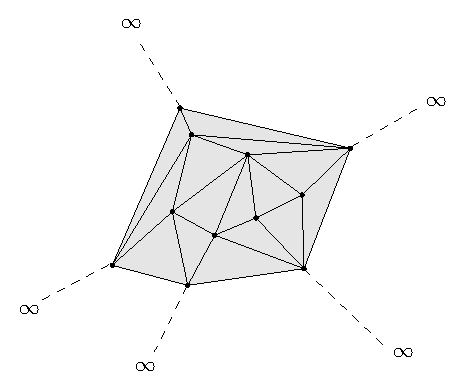
\includegraphics[scale=0.5]{Triangulation_2_ref/infinite_vertex} \end{center}
\end{ccTexOnly}

\begin{ccHtmlOnly}
<CENTER>
<img border=0 src="./infinite_vertex.gif" align=middle alt="Vertices at
infinity">
</CENTER>
\end{ccHtmlOnly}

\caption{The infinite vertex.
\label{Triangulation_ref_Fig_infinite_vertex}}
\end{figure}

The class \ccRefName\
implements this point of view
and therefore considers  the triangulation of the set of points 
as a set of  triangular,  finite and
infinite faces. 
Although it is convenient to draw a triangulation as in
figure~\ref{Triangulation_ref_Fig_infinite_vertex}, note that
the \ccc{infinite vertex} has no significant
coordinates and that no geometric predicate can be applied on it
or on an infinite face.

A triangulation is a collection of vertices and faces that
are linked together through incidence and adjacency relations.
Each face give access to its three incident vertices and to
its 
three adjacent faces. Each vertex give access to one of its  incident
faces. 

The three vertices of a face are indexed with 0, 1 and 2
in counterclockwise order. The neighbor of a face are also 
indexed with 0,1,2 in such a way that the neighbor indexed by $i$
is opposite to the vertex with the same index.

The triangulation class
offer  two functions \ccStyle{int cw(int i)} and 
\ccStyle{int ccw(int i)} 
which given the index of a vertex in a face
compute the index of the next vertex  of the same face
in clockwise
or counterclockwise order.
 Thus, for example the neighbor 
\ccc{neighbor(cw(i))} is
 the
neighbor of \ccc{f}  which is next to \ccc{neighbor(i)} turning clockwise
around \ccc{f}. The face \ccc{neighbor(cw(i))}
is also the first face encountered after \ccc{f} when
turning clockwise around vertex \ccc{i}
of~\ccc{f} (see Figure~\ref{Triangulation_ref_Fig_neighbors}).



 \begin{figure}
\begin{ccTexOnly}
    \begin{center}
     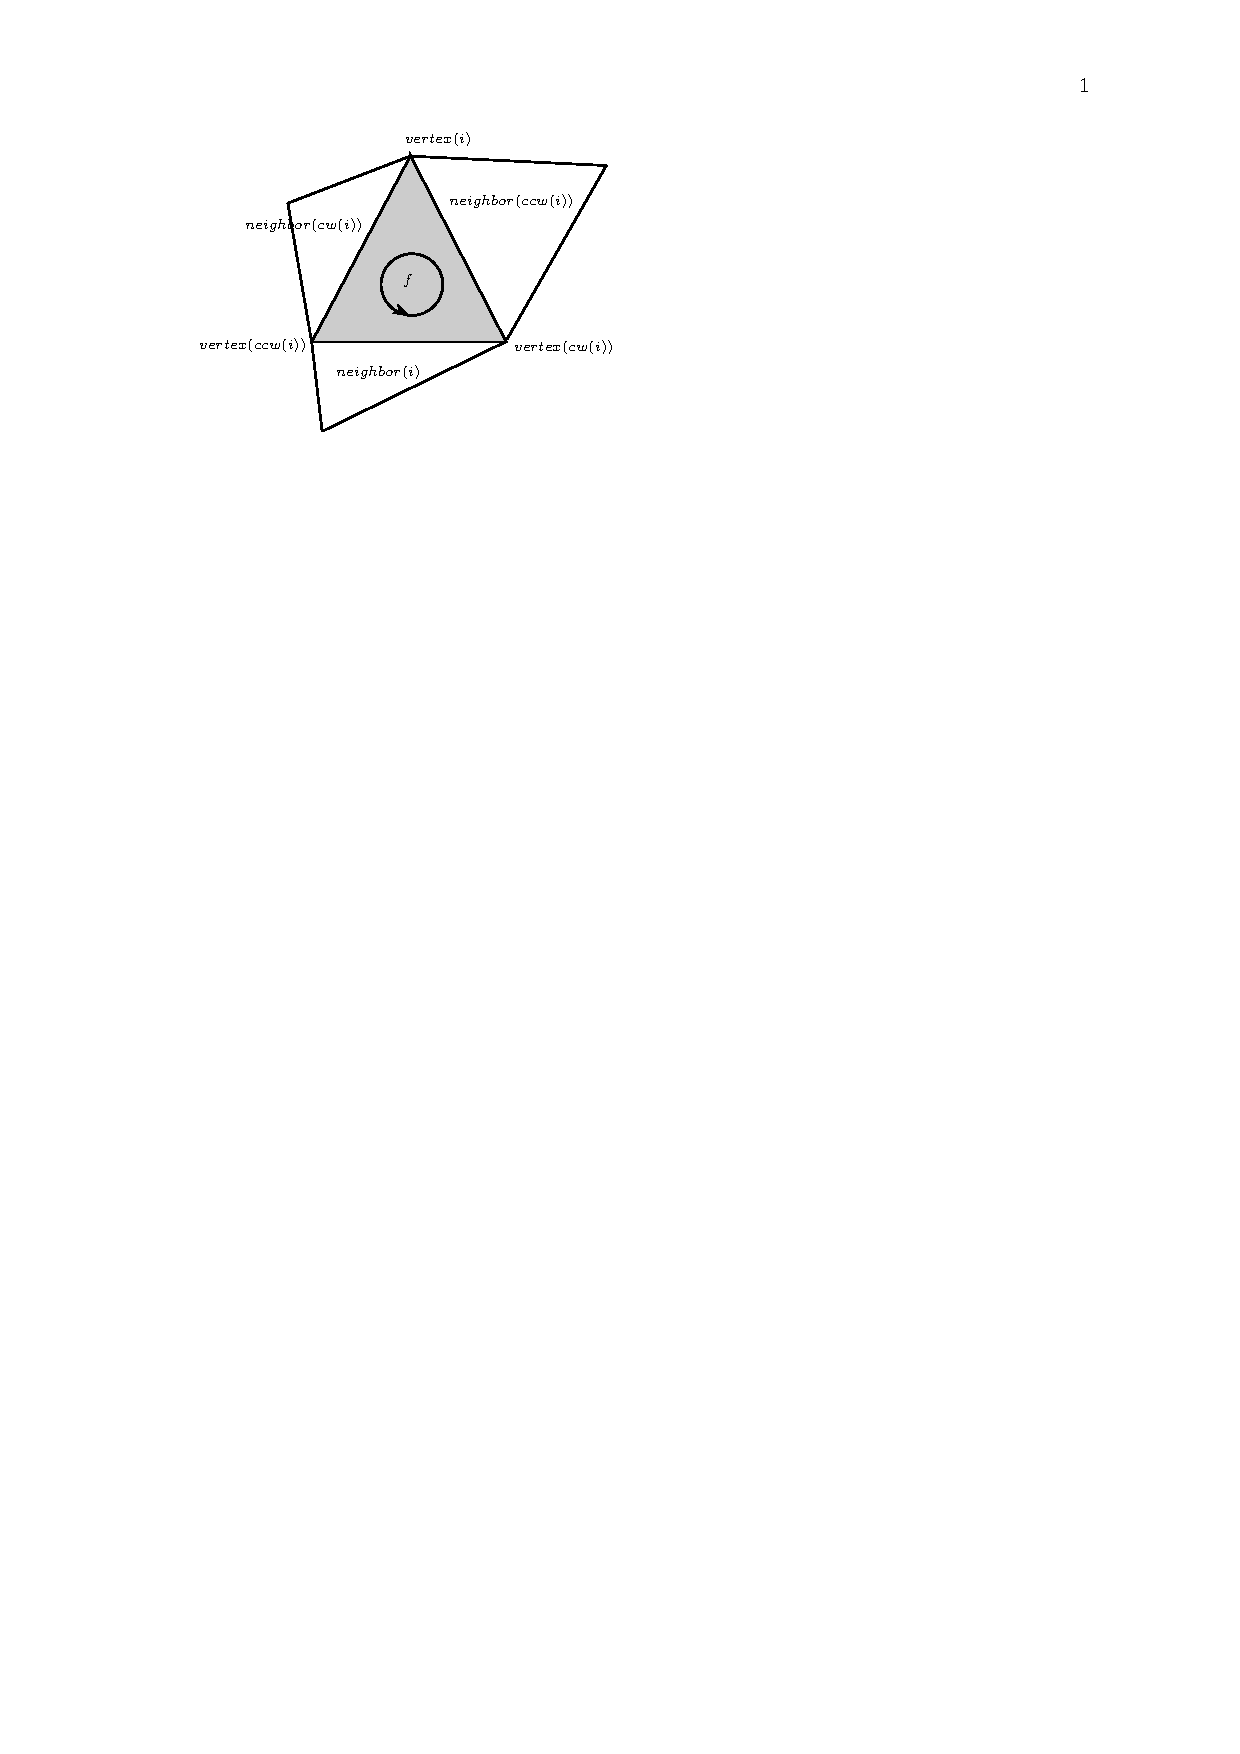
\includegraphics{Triangulation_2/neighbors}
    \end{center}
\end{ccTexOnly} 

  \begin{ccHtmlOnly}
<CENTER>
<img border=0 src="./neighbors.gif" align=middle alt="Neighbors">
</CENTER>
\end{ccHtmlOnly}     

\caption{Vertices and neighbors.
    \label{Triangulation_ref_Fig_neighbors}}
\end{figure}



\ccInclude{CGAL/Triangulation_2.h}

\ccParameters
The class \ccRefName\ has  two template parameters. The first one
\ccc{Traits} is the geometric traits, it is to be instantiated by
 a model of the concept \ccc{TriangulationTraits_2}.

The second parameter is the triangulation data structure,
it has to be instantiated by a model of the concept
\ccc{TriangulationDataStructure_2}.
By default, the triangulation data structure  is instantiated by
\ccc{CGAL::Triangulation_data_structure_2 <
                       CGAL::Triangulation_vertex_base_2<Gt>,
		       CGAL::Triangulation_face_base_2<Gt> > >}.


\ccInheritsFrom{\ccc{Triangulation_cw_ccw_2}}
This class provides the functions \ccc{cw(i)} and \ccc{ccw(i)}.

\ccTypes
\ccThree{typedef Traits::Triangle_2xxx}{Triangulation_data_structure;}{}
\ccTypedef{typedef Traits Geom_traits;}{the traits class.}
\ccGlue
\ccTypedef{typedef Tds Triangulation_data_structure;}{the triangulation data structure type.}

\ccTypedef{typedef Traits::Point_2 Point;}{the point type}
\ccGlue
\ccTypedef{typedef Traits::Segment_2 Segment;}{the segment type}
\ccGlue
\ccTypedef{typedef Traits::Triangle_2 Triangle;}{the triangle type}

\ccTypedef{typedef Tds::Vertex Vertex;}{the vertex type.}
\ccGlue
\ccTypedef{typedef Tds::Face Face;}{the face type.}
\ccGlue
\ccTypedef{typedef Tds::Edge  Edge;} {the edge type.}

\ccTypedef{typedef Tds::size_type size_type;}
{Size type (an unsigned integral type)}
\ccGlue
\ccTypedef{typedef Tds::difference_type difference_type;}
{Difference type (a signed integral type)}

\ccThree{typedef Traits::Triangle_2xxx}{}{the triangulation data structure type}
\ccThreeToTwo
The vertices and faces of the triangulations are accessed through 
\ccc{handles}, 
\ccc{iterators} and \ccc{circulators}. 
The  handles are models of the concept \ccc{Handle} which basically
offers the two dereference operators \ccc{*} and \ccc{->}.
The iterators and circulators
are all bidirectional and non mutable.
The circulators and iterators are convertible  to handles with the
same value type, so that whenever a handle appear in the parameter 
list of a function, an appropriate iterator or circulator can be passed
as well.

The edges of the triangulation can also be visited through iterators
and circulators,
the edge circulators and iterators
are also bidirectional and non mutable.

In the following, we called {\it infinite} any face or edge 
incident  to the infinite vertex and the infinite vertex itself.
 Any other feature (face, edge or vertex) of the triangulation is said 
to be {\it finite}.
Some iterators (the \ccc{All} iterators ) allows to visit finite or 
infinite feature while others (the \ccc{Finite} iterators) visit only
finite features. Circulators visit infinite features as well as finite 
ones.

\ccTypedef{typedef Tds::Vertex_handle Vertex_handle;}
{handle to a vertex}
\ccGlue
\ccTypedef{typedef Tds::Face_handle Face_handle;}
{handle to a face}


\ccTypedef{typedef Tds::Face_iterator All_faces_iterator;}
{iterator over all faces.}
\ccGlue
\ccTypedef{typedef Tds::Edge_iterator All_edges_iterator;}
{iterator over all edges}
\ccGlue
\ccTypedef{typedef Tds::Vertex_iterator All_vertices_iterator;}
{iterator over all vertices}

\ccNestedType{Finite_faces_iterator}{iterator over finite faces.}
\ccGlue
\ccNestedType{Finite_edges_iterator
}{iterator over finite edges.}
\ccGlue
\ccNestedType{Finite_vertices_iterator}{iterator over finite
vertices.}
\ccGlue
\ccNestedType{Point_iterator}{iterator over the points corresponding the
finite vertices of the triangulation.} 


\ccNestedType{Line_face_circulator}{circulator over all faces intersected by a line.}


\ccNestedType{Face_circulator} 
{circulator over all faces incident to a given vertex.}
\ccGlue
\ccNestedType{Edge_circulator}
{circulator over all  edges incident to a given vertex.}
\ccGlue
\ccNestedType{Vertex_circulator}
{circulator over all vertices incident to a given vertex.}

The triangulation class also defines the following enum type to specify
which case occurs when locating a point in the triangulation.

\ccEnum{enum Locate_type {VERTEX=0, EDGE, FACE, OUTSIDE_CONVEX_HULL,
OUTSIDE_AFFINE_HULL};}{The locate type is \ccc{OUTSIDE_CONVEX_HULL} when the point
is  outside the convex hull but in the affine hull of the current triangulation. \\
The locate type is \ccc{OUTSIDE_AFFINE_HULL} 
when the point is outside the affine hull
of the current triangulation.}


\ccCreation
\ccCreationVariable{t}  %% choose variable name



\ccThree{Triangulation_2<>}{t = Triangulation_2 tr}{}
\ccThreeToTwo
\ccConstructor{Triangulation_2();}{default constructor.}
\ccGlue
\ccConstructor{Triangulation_2(
                   const Traits& gt = Traits() );}
{Introduces an empty triangulation \ccVar.}


\ccConstructor{Triangulation_2(
                   const Triangulation_2& tr);}
{Copy constructor. All the vertices and faces are duplicated.
 After the copy, \ccVar\ and \ccc{tr}
refer to different triangulations~: 
 if \ccc{tr} is modified, \ccVar\ is not. }

\ccMethod{Triangulation_2 operator=(const Triangulation_2<Traits,Tds>& tr);}
{Assignment. All the vertices and faces are duplicated.
 After the assignment, \ccVar\ and \ccc{tr}
refer to different triangulations~: 
 if \ccc{tr} is modified, \ccVar\ is not.}

\ccThree{Vertex_handle}{t.number_of_vertices()x}{}
\ccMethod{void swap(Triangulation_2& tr);}
{The triangulations \ccc{tr} and \ccVar\ are swapped.
\ccc{t.swap(tr)} should be preferred to \ccc{t} = \ccc{tr} or to
\ccc{t(tr)} if \ccc{tr} is deleted after that.}

\ccMethod{void clear();}{Deletes all faces and finite vertices
resulting
 in an
empty triangulation.}

%\ccFunction{void ~Triangulation_2();}
%{Destructor. All vertices and faces are deleted.}


\ccAccessFunctions
\ccMethod{const Geom_traits& geom_traits() const;}
{Returns a const reference to the triangulation traits object.}
\ccGlue
\ccMethod{const TriangulationDataStructure_2 & tds() const;}
{Returns a const reference to the triangulation data structure.}

\begin{ccAdvanced}
\ccHeading{Non const access}
The responsibility of keeping a valid triangulation belongs to the user
when using advanced operations allowing a direct manipulation of the \ccc{tds}.

\ccMethod{TriangulationDataStructure_2 & tds();}
{Returns a reference to the triangulation data structure.}

This method is mainly a help for users implementing their own triangulation
algorithms.
 
\end{ccAdvanced}


\ccGlue
\ccMethod{int dimension() const;}
{Returns the dimension of the convex hull.}
\ccGlue
\ccMethod{size_type number_of_vertices() const;}
{Returns the number of finite vertices.}
\ccGlue
\ccMethod{size_type number_of_faces() const;}
{Returns the number of finite faces.}

\ccMethod{Face_handle infinite_face() const;}
{a  face incident to the \ccc{infinite_vertex}.}
\ccGlue
\ccMethod{Vertex_handle
          infinite_vertex();}
{the \ccc{infinite_vertex}.}
\ccGlue
\ccMethod{Vertex_handle finite_vertex() const;}
{a vertex distinct from  the \ccc{infinite_vertex}.}


\ccPredicates
The class \ccRefName\ provides methods to test
the finite or infinite character of any feature,
and also methods to test the presence in the triangulation
of a particular feature (edge or face).

\ccThree{bool }{t.is_infinite( Face_handle f, int i)x}{}
\ccMethod{bool
          is_infinite(Vertex_handle v) const;}
{\ccc{true} iff \ccc{v} is the \ccc{infinite_vertex}.}
\ccGlue
\ccMethod{bool
          is_infinite(Face_handle f) const;}
{\ccc{true} iff face \ccc{f} is infinite.}
\ccGlue
\ccMethod{bool is_infinite(Face_handle f, int i) const;}
{\ccc{true} iff edge \ccc{(f,i)} is infinite.}
\ccGlue
\ccMethod{bool
          is_infinite(Edge e) const;}
{\ccc{true} iff edge \ccc{e} is infinite.}
\ccGlue
\ccMethod{bool
          is_infinite(Edge_circulator ec) const;}
{\ccc{true} iff edge \ccc{*ec} is infinite.}
\ccGlue
\ccMethod{bool
          is_infinite(Edge_iterator ei) const;}
{\ccc{true} iff edge \ccc{*ei} is infinite.}


\ccMethod{bool is_edge(Vertex_handle va, Vertex_handle vb);}
{\ccc{true} if there is an edge having \ccc{va} and \ccc{vb} as
vertices.}
\ccGlue
\ccMethod{bool is_edge(Vertex_handle va, Vertex_handle vb, Face_handle& fr,
	       int & i);}
{ as above. In addition, if \ccc{true} is returned,  the edge with
vertices \ccc{va} and \ccc{vb} is the edge \ccc{e=(fr,i)} where
\ccc{fr} is a handle to the face incident to \ccc{e} and 
on the right side of  \ccc{e} oriented from \ccc{va} to \ccc{vb}.}
\ccGlue
\ccMethod{bool includes_edge(Vertex_handle va, Vertex_handle & vb,
		     Face_handle& fr, int & i);}
{\ccc{true} if the line segment from \ccc{va} to \ccc{vb} includes
an edge \ccc{e} incident to \ccc{va}. If \ccc{true}, \ccc{vb} becomes
the other vertex of \ccc{e}, \ccc{e} is the edge \ccc{(fr,i)} where
\ccc{fr} is a handle to the face incident to \ccc{e} and 
on the right side \ccc{e} oriented from \ccc{va} to \ccc{vb}.}
\ccGlue
\ccMethod{bool is_face(Vertex_handle v1, Vertex_handle v2, Vertex_handle v3);}
{\ccc{true} if there is a face having \ccc{v1}, \ccc{v2} and \ccc{v3} 
as vertices.}
\ccGlue
\ccMethod{bool is_face(Vertex_handle v1, Vertex_handle v2, Vertex_handle v3,
      Face_handle &fr);}
{as above. In addition, if \ccc{true} is returned, fr is a handle
to the face with  \ccc{v1}, \ccc{v2} and \ccc{v3} 
as vertices.} 

\ccHeading{Queries}

The class \ccRefName\  provides methods to locate
a given point with respect to a triangulation. It also provides
methods to locate a point with respect to
a given  finite face of the triangulation.

\ccThree{Vertex_handle}{t.locate(Point query,}{}
\ccMethod{Face_handle
          locate(const Point& query,
                 Face_handle f = Face_handle()) const;}
{If the point \ccc{query} lies inside the convex hull of the points, a face 
that contains the query in its interior or on its
 boundary is returned.\\
If the point \ccc{query} lies outside the convex hull of the
triangulation but in the affine hull,
the returned face is an infinite face which is a proof of the point's
location : \\
- for a two dimensional triangulation, it is a face $(\infty, p, q)$ 
such that
\ccc{query} lies to the left  of the oriented line $pq$ 
(the rest of the triangulation lying to the right of this line).\\
- for a degenerate one dimensional triangulation it is the (degenerate
one dimensional) face $(\infty, p, NULL)$ such that \ccc{query}
and the triangulation lie on either side of \ccc{p}. \\
If the point \ccc{query} lies outside the affine hull,
the returned \ccc{Face_handle} is \ccc{NULL}. \\
The optional \ccc{Face_handle} argument, if provided, is used as a hint
of where the locate process has to start its search.}

\ccMethod{Face_handle
          locate(const Point& query,
                 Locate_type& lt,
                 int& li,
                 Face_handle h =Face_handle() ) const;}
{Same as above. Additionally, the parameters \ccc{lt}
 and \ccc{li}
describe where the query point is located. 
The variable \ccc{lt} is set to the locate type of the query.
If \ccc{lt==VERTEX} 
the variable \ccc{li}
is set to the index of the vertex, and if \ccc{lt==EDGE}
\ccc{li}
is set to the index 
of the vertex opposite to the
edge. 
Be careful that \ccc{li}
has no meaning when the query type is \ccc{FACE}, \ccc{OUTSIDE_CONVEX_HULL}, 
or \ccc{OUTSIDE_AFFINE_HULL} or when the
triangulation is $0$-dimensional.}

\ccMethod{Oriented_side
           oriented_side(Face_handle f,
                         const Point& p) const;}
{Returns on which side of the oriented boundary of \ccc{f} lies 
the point \ccc{p}. \ccPrecond \ccc{f} is finite.}

\ccMethod{Oriented_side
 side_of_oriented_circle(Face_handle f, const Point & p);}
{Returns on which side of the circumcircle  of face \ccc{f} lies 
the point \ccc{p}. The circle is assumed to be counterclockwise
oriented, so its positive
side correspond to its bounded side.
This predicate is available only if the corresponding predicates on
points is provided in the geometric traits class.}

\ccHeading{Modifiers}

The following operations are guaranteed to lead to a valid triangulation 
when they are applied on a valid triangulation.

\ccMethod{void flip(Face_handle f, int i);}{Exchanges the edge incident to
\ccc{f} and \ccc{f->neighbor(i)} with the other
diagonal of the quadrilateral formed by \ccc{f} and  \ccc{f->neighbor(i)}.
\ccPrecond {The faces \ccc{f} and \ccc{f->neighbor(i)} are finite faces
and their union form a convex quadrilateral.}}



\ccMethod{Vertex_handle insert(const Point& p,
                         Face_handle f = Face_handle());}
{Inserts point \ccc{p} in the triangulation and returns the corresponding
 vertex.\\
If point \ccc{p} coincides with an already existing vertex, this 
vertex is returned and the triangulation remains unchanged.\\
If point \ccc{p} is on an edge, the two incident faces are split 
in two.\\
If point \ccc{p} is strictly inside a face of the triangulation,
the face is split in three.\\
If point \ccc{p} is strictly outside the  convex hull, \ccc{p} is linked
to all visible points on the convex hull to form the new
triangulation.\\
At last, if \ccc{p} is outside the affine hull (in case of degenerate
1-dimensional or 0-dimensional triangulations), \ccc{p}
is linked all the  other vertices to form a triangulation whose
dimension is increased by one.
The last argument \ccc{f} is an indication to the underlying locate
algorithm of where to start.
}


\ccMethod{Vertex_handle 
          insert(const Point& p,
                 Locate_type lt,
                 Face_handle loc, int li );}
{Same as above except that the location of the point
 \ccc{p} to be inserted is assumed to be given by
\ccc{(lt,loc,i)} (see the description of the \ccc{locate} method above.)}

\ccMethod{Vertex_handle push_back(const Point& p);}
{Equivalent to \ccc{insert(p)}.}

\ccMethod{template < class InputIterator >
          size_type
          insert(InputIterator first, InputIterator last);}
{Inserts the points in the range
 $\left[\right.$\ccc{first}, \ccc{last}$\left.\right)$.
 Returns the number of inserted points.
 \ccPrecond The \ccc{value_type} of \ccc{InputIterator}
 is \ccc{Point}.}

\ccMethod{void    remove(Vertex_handle v);}
{Removes the vertex from the triangulation. The created hole is 
 re-triangulated.
 \ccPrecond Vertex \ccc{v} must be finite.}

\ccMethod{Vertex_handle    move_if_no_collision(Vertex_handle v, const Point & p);}
{if there is not already another vertex placed on \ccc{p}, 
the triangulation is modified such that the new position of vertex \ccc{v}
is \ccc{p}, and \ccc{v} is returned. Otherwise, the triangulation is not
modified and the vertex at point \ccc{p} is returned.
\ccPrecond Vertex \ccc{v} must be finite.}

\ccMethod{Vertex_handle    move(Vertex_handle v, const Point & p);}
{same as above if there is no collision. Otherwise, \ccc{v}
is deleted and the vertex placed on \ccc{p} is returned.
 \ccPrecond Vertex \ccc{v} must be finite.}

\begin{figure}
\begin{ccTexOnly}
\begin{center}
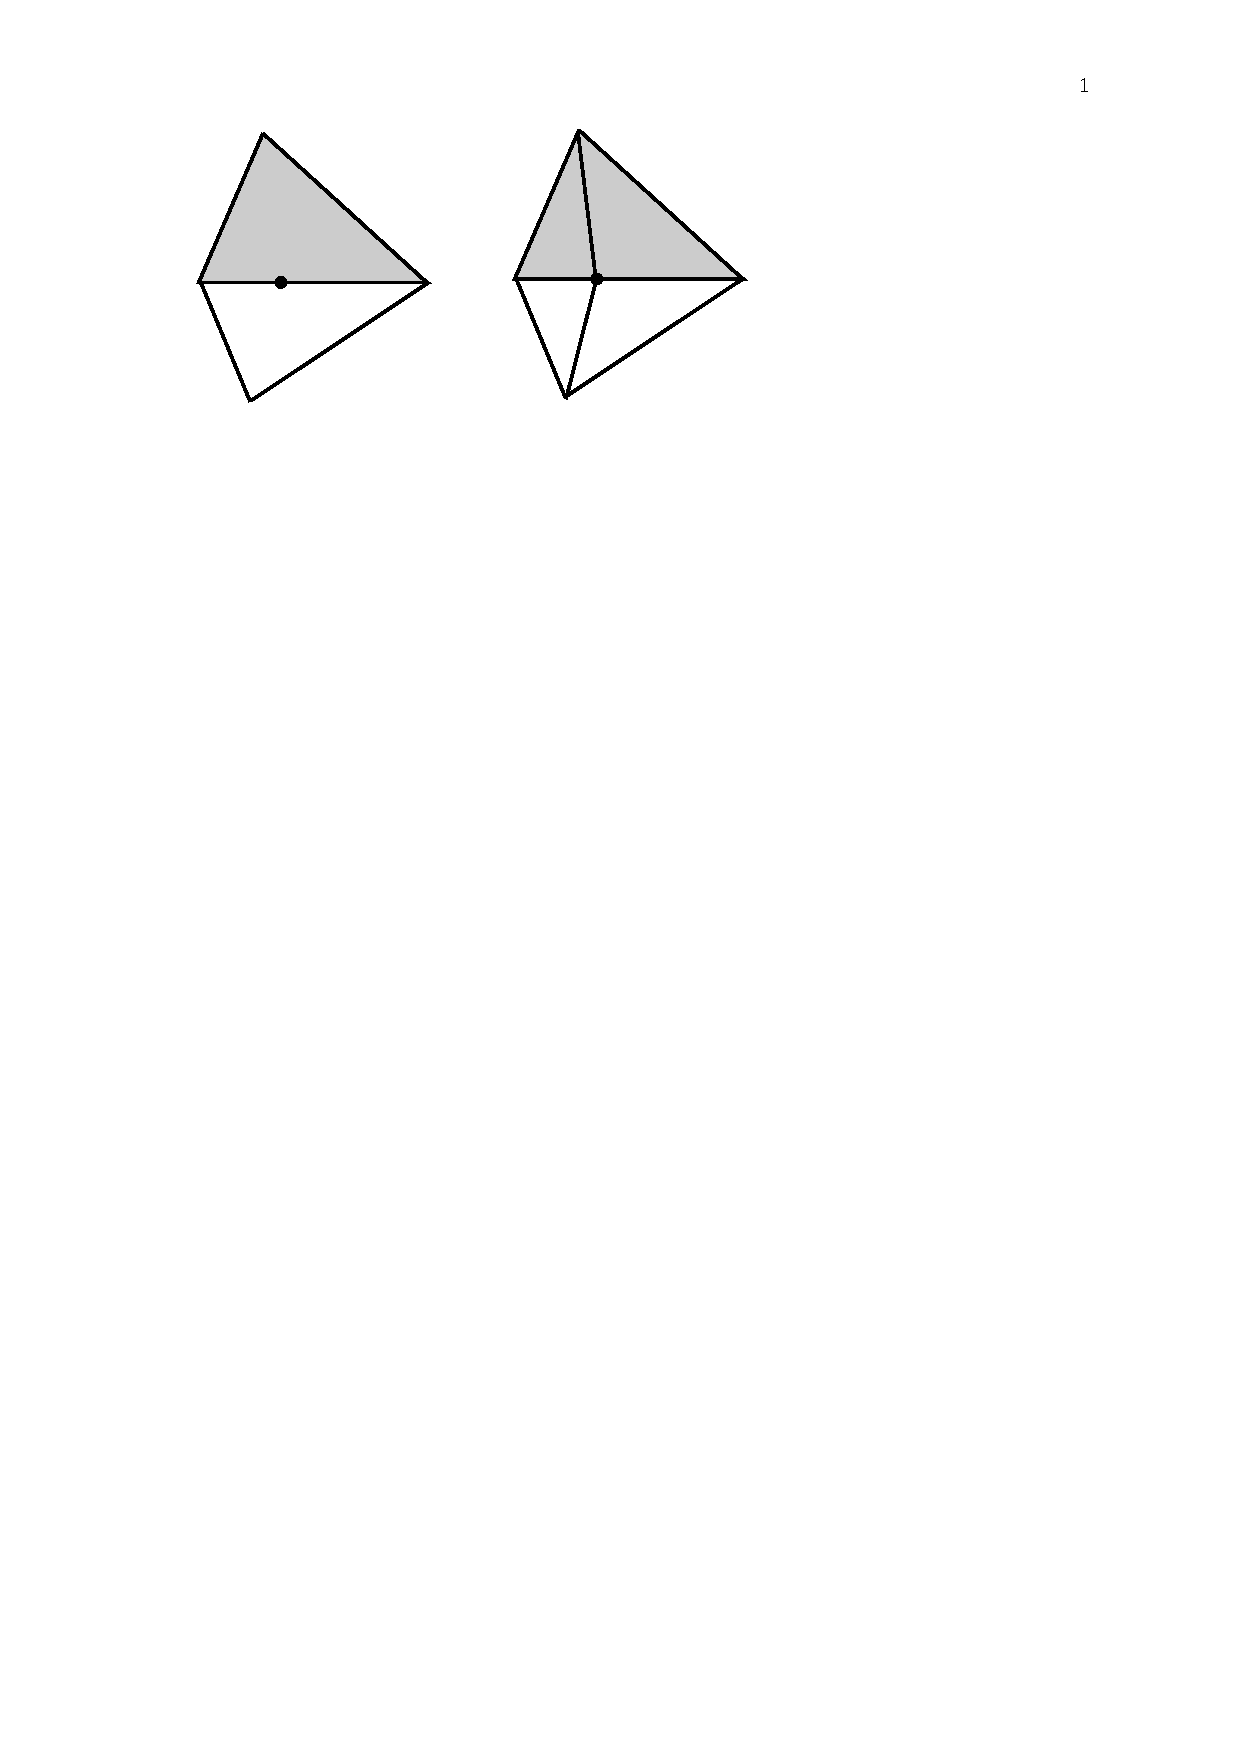
\includegraphics{Triangulation_2/insert1}
\end{center}
\end{ccTexOnly}


\begin{ccHtmlOnly}
<CENTER>
<img border=0 src="./insert1.gif" align=middle alt="Insertion in an edge">
</CENTER>
\end{ccHtmlOnly}

\caption{Insertion of a point on an edge.
\label{Triangulation_ref_Fig_inser1t}}
\end{figure}




\begin{figure}
\begin{ccTexOnly}
\begin{center}
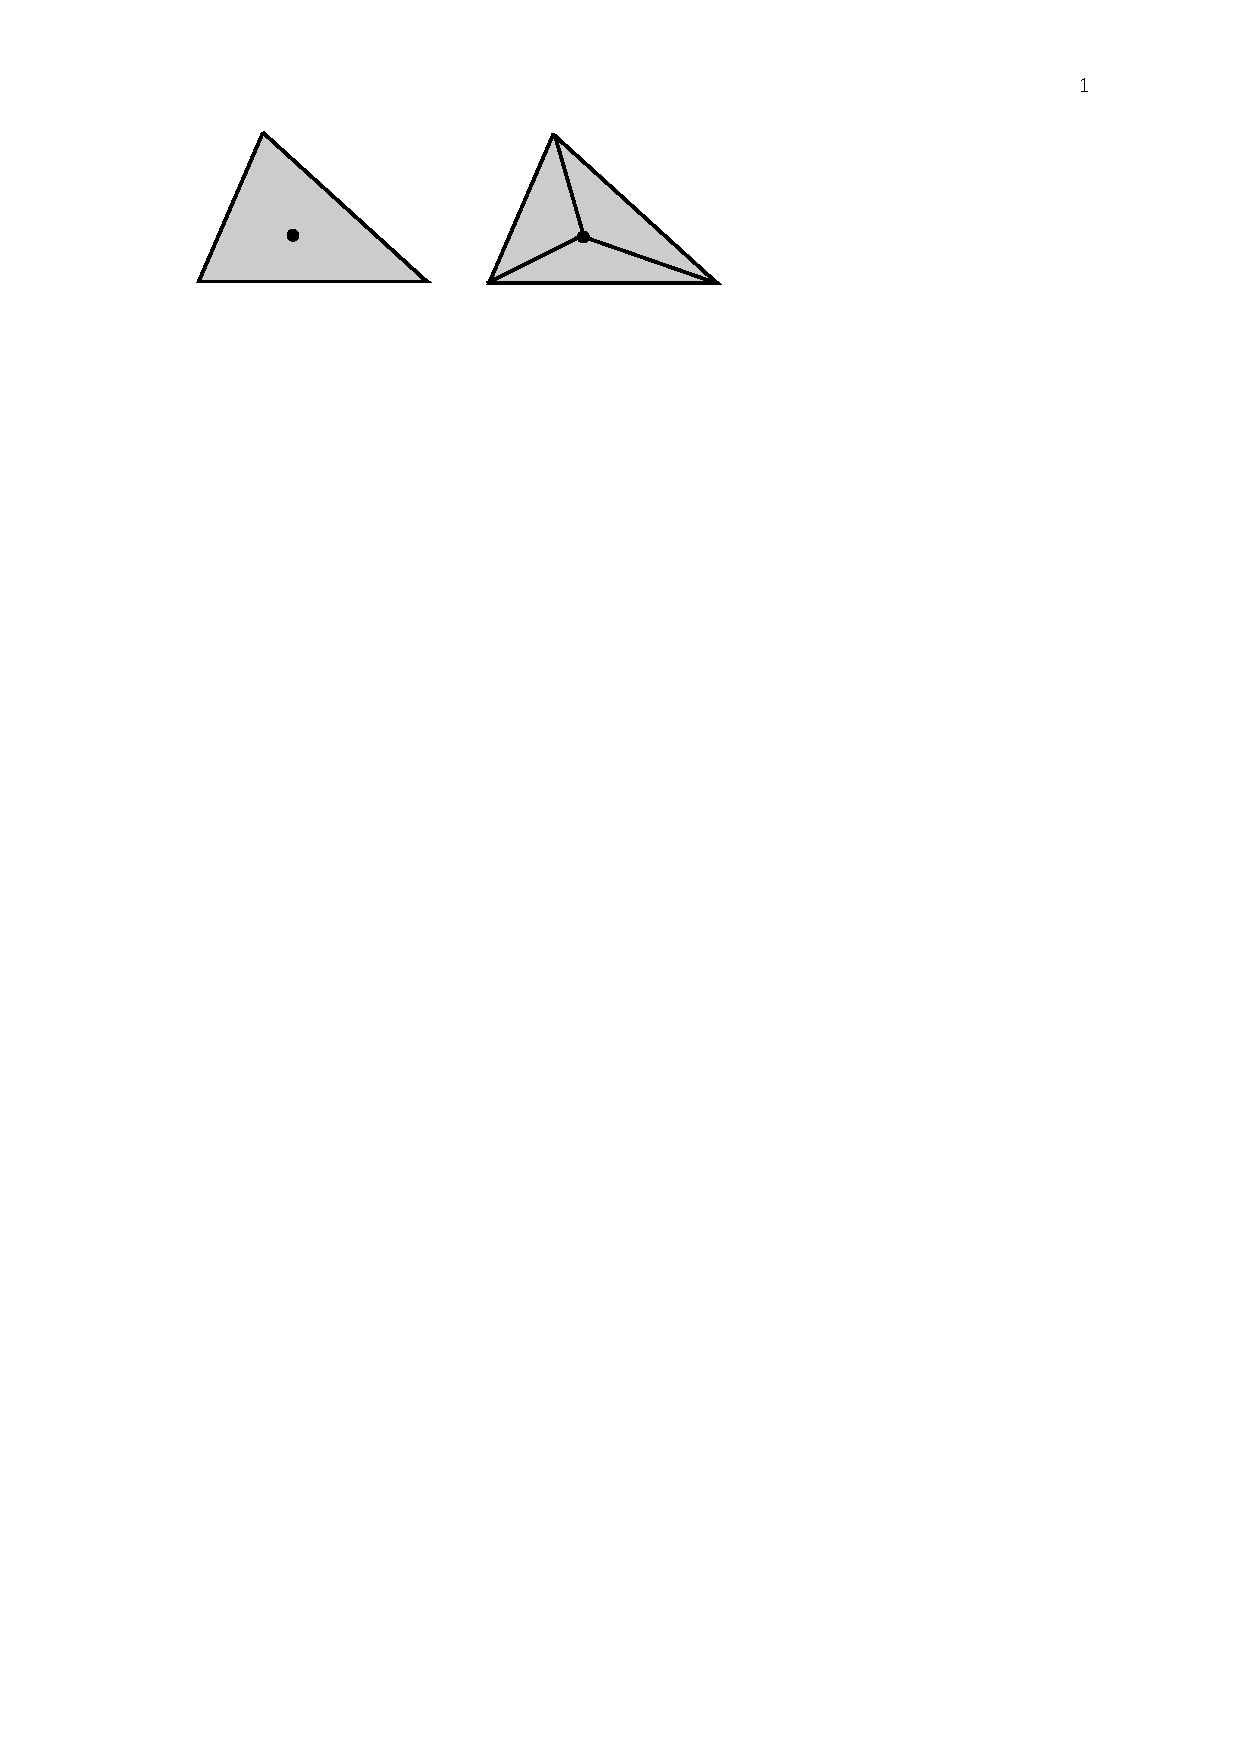
\includegraphics{Triangulation_2/insert2}
\end{center}
\end{ccTexOnly}

\begin{ccHtmlOnly}
<CENTER>
<img border=0 src="./insert2.gif" align=middle alt="Insertion in a Face">
</CENTER>
\end{ccHtmlOnly}

\caption{Insertion in a face.
\label{Triangulation_ref_Fig_insert2}}

\end{figure}


\begin{figure}
\begin{ccTexOnly}
\begin{center}
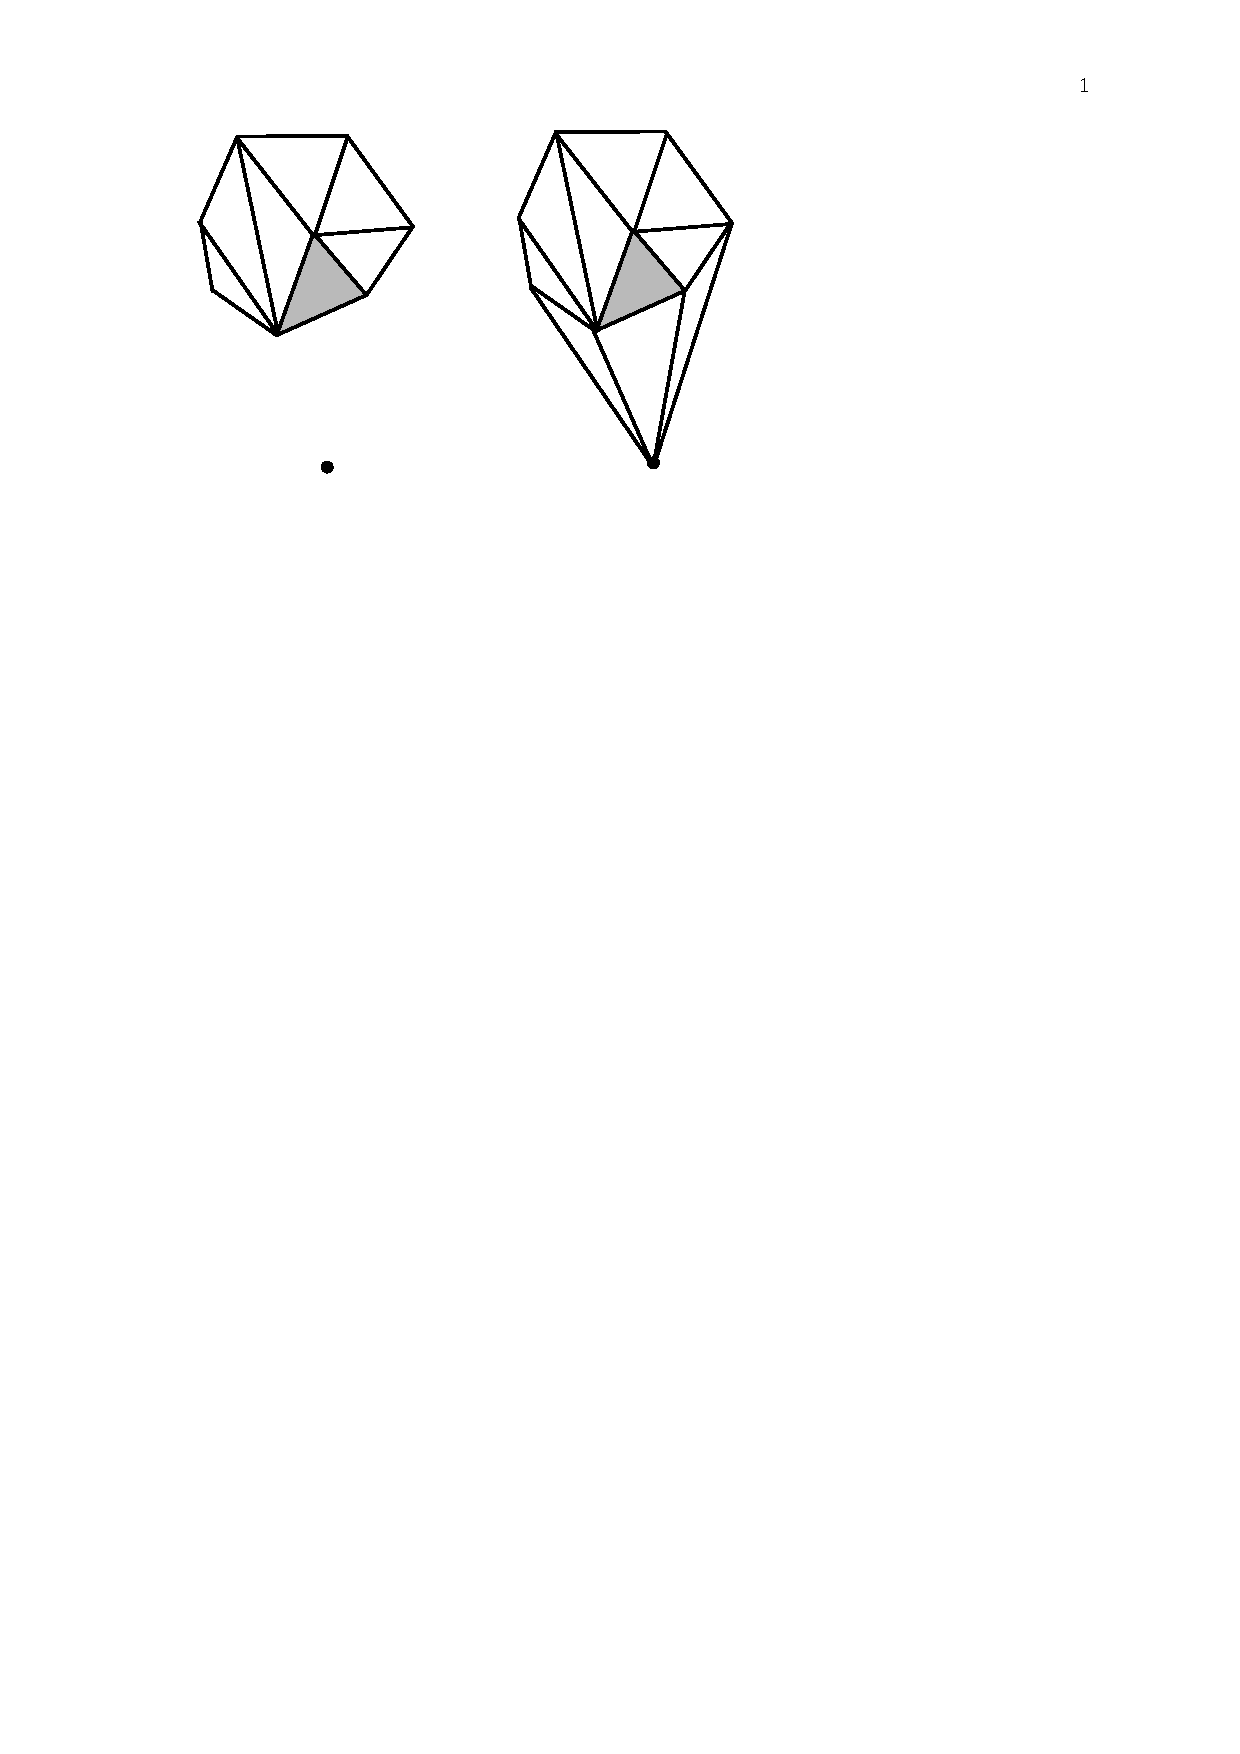
\includegraphics{Triangulation_2/insert3}
\end{center}
\end{ccTexOnly}


\begin{ccHtmlOnly}
<CENTER>
<img border=0 src="./insert3.gif" align=middle alt="Insertion outside the
convex hull">
</CENTER>
\end{ccHtmlOnly}

\caption{Insertion outside the convex hull.
\label{Triangulation_ref_Fig_insert3}}
\end{figure}

\begin{figure}
\begin{ccTexOnly}
\begin{center}
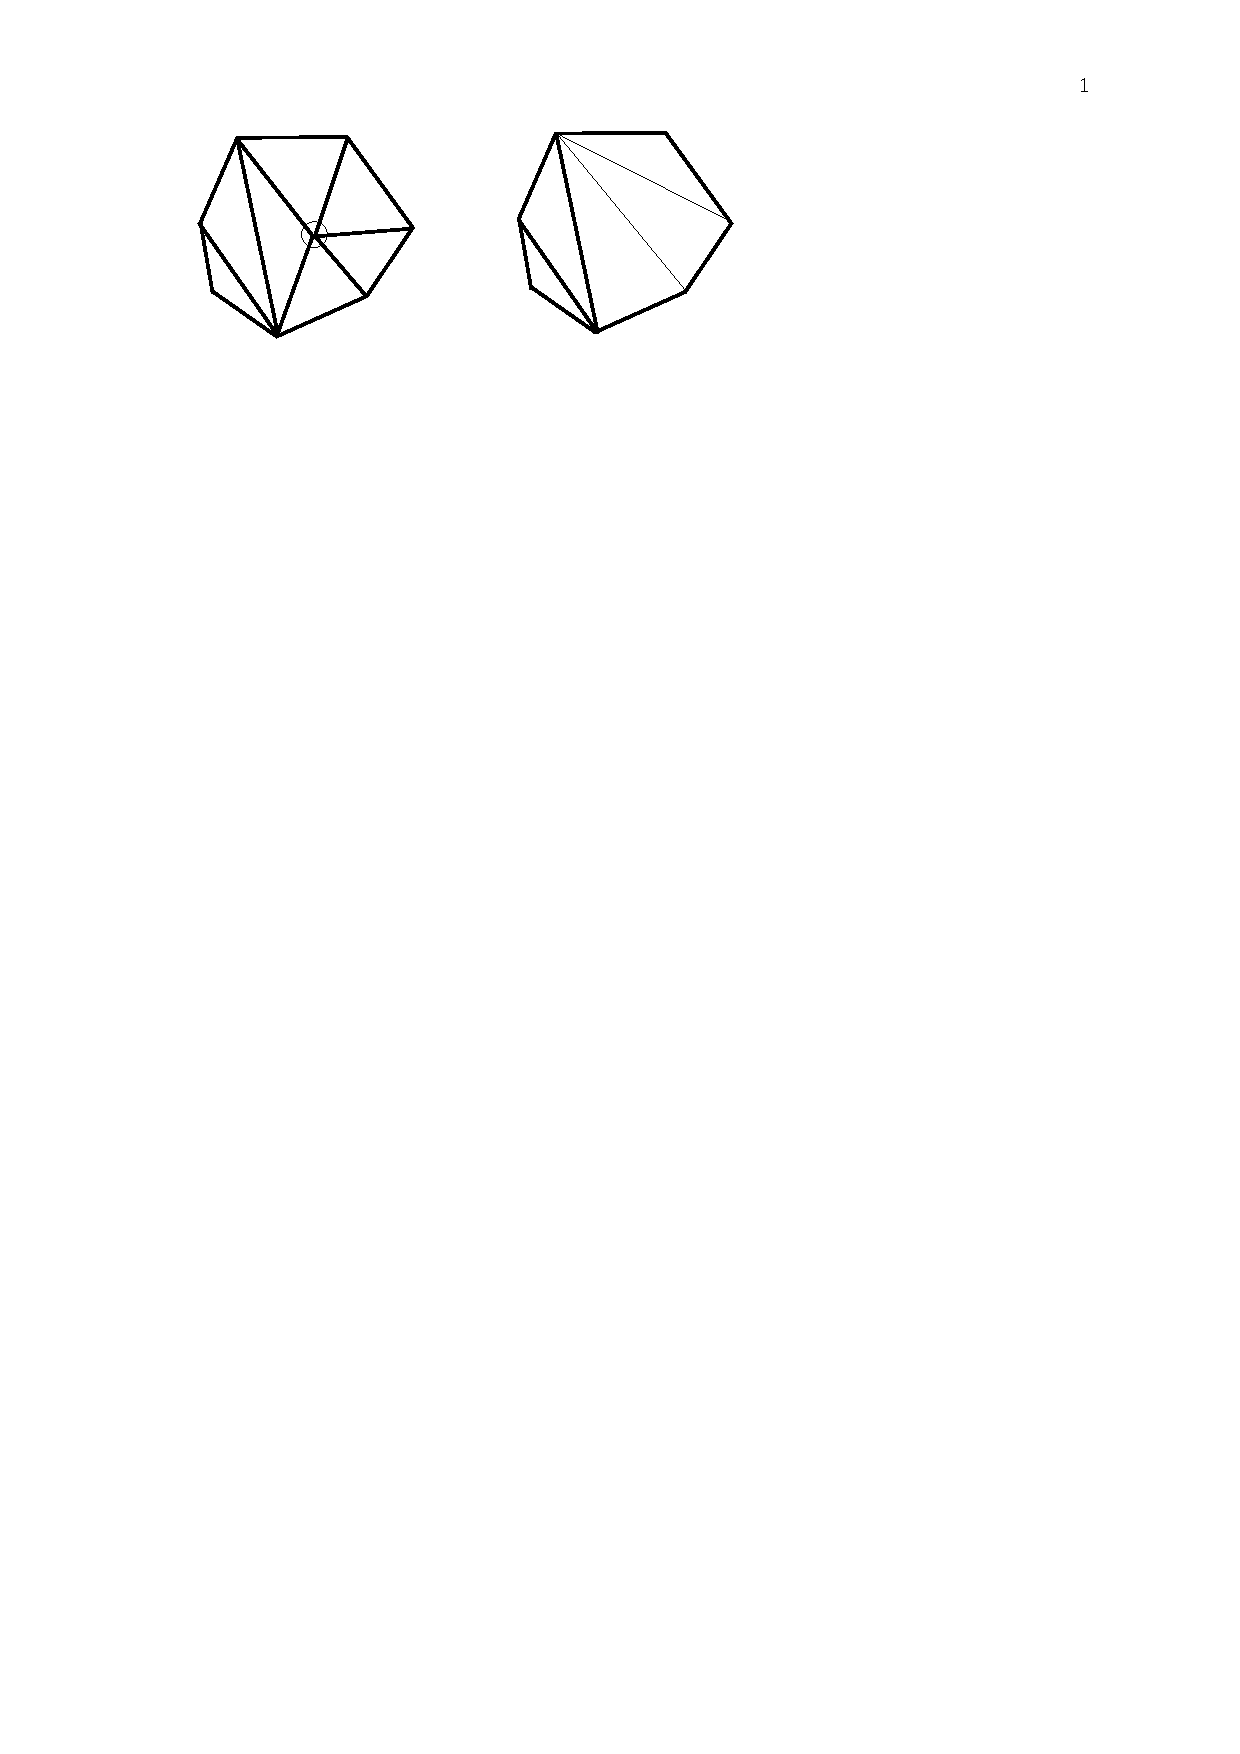
\includegraphics{Triangulation_2/remove}
\end{center}
\end{ccTexOnly}

\begin{ccHtmlOnly}
<CENTER>
<img border=0 src="./remove.gif" align=middle alt="Remove">
</CENTER>
\end{ccHtmlOnly}

\caption{Removal
\label{Triangulation_ref_Fig_remove}}
\end{figure}

\begin{ccAdvanced}
The following member functions offer more specialized versions of the
insertion or removal operations to be used when one knows to be in the
corresponding case.

\ccMethod{Vertex_handle insert_first(const Point& p);} 
{Inserts the first finite  vertex .}
\ccMethod{Vertex_handle insert_second(const Point& p);} 
{Inserts the second finite  vertex .}
\ccMethod{Vertex_handle insert_in_face(const Point& p,Face_handle f);} {Inserts vertex \ccc{v} in face
\ccc{f}. Face \ccc{f} is modified,
two new faces are created.
\ccPrecond{The point in vertex \ccc{v} lies inside face \ccc{f}.}}
\ccMethod{Vertex_handle insert_in_edge(const Point& p, Face_handle f, int i);} 
{Inserts vertex v in edge \ccc{i} of \ccc{f}.
\ccPrecond{The point in vertex \ccc{v} lies on the edge opposite to 
the vertex \ccc{i} of face \ccc{f}.}}
\ccMethod{Vertex_handle insert_outside_convex_hull(const Point& p, Face_handle f);}
{Inserts 
 a point which is outside the convex hull  but in the affine hull.
\ccPrecond{
The handle \ccc{f} points to a face which is a proof  of the location
of\ccc{p}, see the description of the
\ccc{locate} method above.} }
\ccMethod{Vertex_handle insert_outside_affine_hull(const Point& p);}
{Inserts 
 a point which is outside the affine hull.}

\ccMethod{void remove_degree_3(Vertex_handle v);}
{Removes a vertex of degree three. Two of the incident faces are destroyed,
the third one is modified.
\ccPrecond{Vertex
\ccc{v} is a finite vertex with degree three.}}
\ccMethod{void remove_second(Vertex_handle v);}{Removes the before last finite vertex.}
\ccMethod{void remove_first(Vertex_handle v);}{Removes the last finite vertex.}

The following functions are mainly intended to be used in conjunction
with the \ccc{find_conflicts()} member functions of Delaunay and constrained 
Delaunay triangulations to perform insertions.

\ccMethod{   template<class EdgeIt>
   Vertex_handle star_hole( Point p, 
 			      EdgeIt edge_begin,
 			      EdgeIt edge_end);}
{creates a new vertex \ccc{v} and use it to star the hole 
whose boundary is described  by the sequence of edges \ccc{[edge_begin, 
edge_end[}. Returns a handle to the new vertex.}

\ccMethod{
   template<class EdgeIt, class FaceIt>
   Vertex_handle star_hole( Point p, 
 			      EdgeIt edge_begin,
 			      EdgeIt edge_end,
 			      FaceIt face_begin,
 			      FaceIt face_end);}
{same as above, except that the  algorithm 
first recycles faces in the sequence \ccc{[face_begin, 
face_end[} 
and create new ones only when the sequence is exhausted.}
\end{ccAdvanced}


\ccHeading{Traversal of the Triangulation}


A triangulation can be seen as a container of faces and vertices.
Therefore the triangulation provides several iterators and circulators
that allow to traverse it (completely or partially).



\ccHeading{Face, Edge and Vertex Iterators}

The following iterators allow respectively to visit 
finite faces,  finite edges and  finite vertices
of the triangulation. These iterators are non mutable, bidirectional
and their value types are respectively
\ccc{Face}, \ccc{Edge} and \ccc{Vertex}. 
They are all invalidated by any change in the triangulation.

\ccThree{Finite_vertices_iterator}{t.finite_vertices_begin()x}{}
\ccMethod{Finite_vertices_iterator finite_vertices_begin() const;}{Starts at an arbitrary finite vertex}
\ccGlue
\ccMethod{Finite_vertices_iterator finite_vertices_end() const;}{Past-the-end iterator}

\ccMethod{Finite_edges_iterator finite_edges_begin() const;}{Starts at an arbitrary finite edge}
\ccGlue
\ccMethod{Finite_edges_iterator finite_edges_end() const;}{Past-the-end iterator}

\ccMethod{Finite_faces_iterator finite_faces_begin() const;}{Starts at an arbitrary finite face}
\ccGlue
\ccMethod{Finite_faces_iterator finite_faces_end()
const;}{Past-the-end iterator}
\ccGlue
\ccMethod{Point_iterator points_begin() const;}{}
\ccGlue
\ccMethod{Point_iterator points_end() const;}{Past-the-end iterator}

The following iterators allow respectively to visit all
(finite or infinite) faces, edges and vertices
of the triangulation. These iterators are non mutable, bidirectional
and their value types are respectively
\ccc{Face}, \ccc{Edge} and \ccc{Vertex}. 
They are all invalidated by any change in the triangulation.


\ccMethod{All_vertices_iterator all_vertices_begin() const;}{Starts at an arbitrary  vertex}
\ccGlue
\ccMethod{All_vertices_iterator all_vertices_end() const;}{Past-the-end iterator}

\ccMethod{All_edges_iterator all_edges_begin() const;}{Starts at an arbitrary edge}
\ccGlue
\ccMethod{All_edges_iterator all_edges_end() const;}{Past-the-end iterator}

\ccMethod{All_faces_iterator all_faces_begin() const;}{Starts at an arbitrary face}
\ccGlue
\ccMethod{All_faces_iterator all_faces_end() const;}{Past-the-end iterator}

\ccThree{Line_face_circulator}{T.line_walk(Point p, }{}
\ccHeading{Line Face Circulator}

The triangulation defines a circulator that allows
to visit all faces that are intersected by a line. 
A  face  \ccc{f} is 
considered has being intersected by 
 the oriented line \ccc{l} if either:
\begin{itemize}\ccTexHtml{\itemsep0pt}{}
\item 
\ccc{f} is a finite face whose interior intersects \ccc{l}, or
\item
 \ccc{f} is a finite face with  an edge collinear with \ccc{l} and lies
to the left of \ccc{l}, or
\item
\ccc{f} is an infinite face incident to a  convex hull edge 
whose interior is intersected
by \ccc{l}, or
\item
\ccc{f} is an infinite face incident to a  convex hull vertex
lying on  \ccc{l} and the finite edge of \ccc{f}
lies to the left of \ccc{l}. 
\end{itemize}
The circulator has a singular value if  the line \ccc{l}
intersect no finite face of the triangulation.
This circulator is
non-mutable and bidirectional. Its value type is \ccc{Face}.

\ccMethod{Line_face_circulator
          line_walk(const Point& p,
                    const Point& q,
                    Face_handle f = Face_handle()) const;}
{ This function returns a circulator that allows to visit the 
 faces intersected by the line \ccc{pq}. 
If there is no such face the circulator has a singular value.\\
 The starting point of the circulator is the face \ccc{f}, or
 the first finite face traversed by \ccc{l} , if
 \ccc{f} is omitted. \\
  The circulator wraps around the \ccc{infinite_vertex} :
after the last traversed finite face, it steps through the infinite face adjacent
to this face then through the infinite face adjacent to the first
traversed finite face then through the first finite traversed face
again.
\ccPrecond The triangulation must have dimension 2.
\ccPrecond Points \ccc{p} and \ccc{q} must be different points.
\ccPrecond If \ccc{f != NULL}, it must point to a finite face
 and the point \ccc{p} must be
inside or on the boundary of \ccc{f}.}

Figure~\ref{Triangulation_ref_Fig_Line_face_circulator} illustrates which finite faces are enumerated. Lines
$l_1$ and $l_2$ have no face to their left. Lines $l_3$ and $l_4$
have faces to their left. Note that the finite faces that are only vertex
incident to lines $l_3$ and  $l_4$ are not enumerated.

\begin{figure}
\begin{ccTexOnly}
\begin{center}  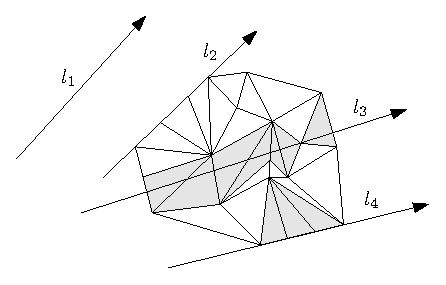
\includegraphics{Triangulation_2/walk} \end{center}
\end{ccTexOnly} 


\begin{ccHtmlOnly}
<CENTER>
<img border=0 src="./walk.gif" align=middle alt="The Infinite Vertex">
</CENTER>
\end{ccHtmlOnly} 

\caption{The line face circulator.
\label{Triangulation_ref_Fig_Line_face_circulator}}
\end{figure}

A line face circulator is invalidated if the face the circulator refers
to is changed.

\ccThree{Vertex_circulator}{t.number_of_vertices()x}{}
\ccThreeToTwo



\ccHeading{Face, Edge and Vertex Circulators}

The triangulation also provides circulators that allows to visit 
respectively all faces or edges incident to a given vertex
or all vertices adjacent to a given vertex.
These circulators are
non-mutable
and bidirectional.
 The \ccc{operator++} moves the circulator
counterclockwise around the vertex while
the \ccc{operator--} moves clockwise.
A face circulator is invalidated by any modification of the face pointed to.
An edge or a vertex circulator are invalidated by any modification
of one of the two faces incident to the edge pointed to.

\ccMethod{Face_circulator incident_faces(Vertex_handle v) const;}
{Starts at an arbitrary face incident
to \ccc{v}.}
\ccGlue
\ccMethod{Face_circulator incident_faces(Vertex_handle v, Face_handle f) const;}
{Starts at face \ccc{f}.
\ccPrecond Face \ccc{f} is incident to vertex \ccc{v}.}
\ccGlue
\ccMethod{Edge_circulator incident_edges(Vertex_handle v) const;}
{Starts at an arbitrary edge incident
to \ccc{v}.}
\ccGlue
\ccMethod{Edge_circulator incident_edges(Vertex_handle v, Face_handle f) const;}
{Starts at the first edge of \ccc{f} incident to 
\ccc{v}, in counterclockwise order around \ccc{v}.
\ccPrecond Face \ccc{f} is incident to vertex \ccc{v}.}
\ccGlue
\ccMethod{Vertex_circulator incident_vertices(Vertex_handle v) const;}
{Starts at an arbitrary  vertex incident
to \ccc{v}.}
\ccGlue
\ccMethod{Vertex_circulator incident_vertices(Vertex_handle v, Face_handle f) ;}
{Starts at the first vertex of \ccc{f} adjacent  to \ccc{v}
in  counterclockwise order around \ccc{v}.
\ccPrecond Face \ccc{f} is incident to vertex \ccc{v}.}




\ccHeading{Traversal of the Convex Hull}

Applied on the \ccc{infinite_vertex}
the above  functions  allow to visit the vertices on the convex hull and
the infinite edges and faces. Note that a counterclockwise
traversal of the vertices adjacent to the \ccc{infinite_vertex} is
a clockwise traversal of the convex hull.

\ccMethod{Face_circulator incident_faces(t.infinite_vertex()) const;}{}
\ccGlue
\ccMethod{Face_circulator incident_faces(t.infinite_vertex(), Face_handle f) const;}{}
\ccGlue
\ccMethod{Edge_circulator incident_edges(t.infinite_vertex()) const;}{}
\ccGlue
\ccMethod{Edge_circulator incident_edges(t.infinite_vertex(), Face_handle f);}{}
\ccGlue
\ccMethod{Vertex_circulator incident_vertices(t.infinite_vertex() v) ;} {}
\ccGlue
\ccMethod{Vertex_circulator incident_vertices(t.infinite_vertex(), Face_handle f) ;}{}

\ccHeading{Traversal between adjacent faces}
\ccMethod{Vertex_handle  mirror_vertex(Face_handle f, int i) const;}
{returns the vertex of the $i^{th}$ neighbor of \ccc{f} that is
  opposite to \ccc{f}.
  \ccPrecond $0\leq i \leq 2$.}

\ccMethod{int   mirror_index(Face_handle f, int i) const;}
{returns the index of \ccc{f} in its $i^{th}$ neighbor.
  \ccPrecond $0\leq i \leq 2$.}



\ccHeading{Miscellaneous}

\ccThree{Segment}{t.segment(Face_handle f, int i); }{}
\ccMethod{int ccw(int i) const;}
{Returns $i+1$ modulo 3.\ccPrecond $0\leq i \leq 2$.}
\ccGlue
\ccMethod{int cw(int i) const;}
{Returns $i+2$ modulo 3.\ccPrecond $0\leq i \leq 2$.}
\ccGlue
%\ccMethod{int number_of_faces() const;}
%{Returns the number of finite and infinite faces.
%\ccc{TBC_TO} Returns the number of finite faces. This access number functions
%%requires to count the degree 
%of the \ccc{infinite_vertex} and thus is not a constant time access function.}
%\ccGlue
\ccMethod{Triangle
          triangle(Face_handle f) const;}
{Returns the triangle formed by the three vertices of \ccc{f}.
 \ccPrecond The face is finite.}
\ccGlue
\ccMethod{Segment
          segment(Face_handle f, int i) const;}
{Returns the line segment formed by the vertices \ccc{ccw(i)}
 and \ccc{cw(i)} of face \ccc{f}.
\ccPrecond $0\leq i \leq 2$. The vertices \ccc{ccw(i)}
 and \ccc{cw(i)} of  \ccc{f}
 are finite.}
\ccGlue
\ccMethod{Segment
          segment(const Edge& e) const;}
{Returns the line segment corresponding to edge \ccc{e}.
\ccPrecond \ccc{e} is a finite edge}
\ccGlue
\ccMethod{Segment
          segment(const Edge_circulator& ec) const;}
{Returns the line segment corresponding to edge \ccc{*ec}.
\ccPrecond \ccc{*ec} is a finite edge.}
\ccGlue
\ccMethod{Segment
          segment(const Edge_iterator& ei) const;}
{Returns the line segment corresponding to edge \ccc{*ei}.
\ccPrecond \ccc{*ei} is a finite edge.}
\ccGlue
\ccMethod{Point circumcenter(Face_handle  f) const;}
{Compute the circumcenter of the face pointed to by f. This function
is available only if the corresponding function is provided in the
geometric traits.}

\begin{ccAdvanced}
\ccHeading{Setting}
\ccMethod{void set_infinite_vertex(const Vertex_handle&  v);}{}

\ccHeading{Checking}
The responsibility of keeping a valid triangulation
belongs to the users if advanced operations are used.
Obviously the advanced user, who implements higher levels operations
may have to make a triangulation invalid at some times. The following
method is provided to help the debugging.

\ccMethod{bool
          is_valid(bool verbose = false, int level = 0) const;}
{Checks the combinatorial validity of the triangulation and
also the validity of its geometric embedding.
 This method is  mainly a debugging help
for the users of advanced features.
}
\end{ccAdvanced}


\ccHeading{I/O}


The I/O operators are defined for \ccc{iostream}.
The format for the iostream
is an internal format. 

%\ccInclude{CGAL/IO/ostream_2.h}

\ccThree{ostream&x}{ostream& os << T}{}
\ccFunction{ostream& operator<<(ostream& os,
                  const Triangulation_2<Traits,Tds>& T);}
{Inserts the triangulation \ccVar\ into the stream \ccc{os}.
\ccPrecond The insert operator must be defined for \ccc{Point}.}

\ccFunction{istream& operator>>(istream& is,
                  const Triangulation_2<Traits,Tds>& T);}
{Reads a triangulation from stream \ccc{is} and assigns it
to \ccVar. \ccPrecond The extract operator must be defined for \ccc{Point}.}

The information output  in the \ccc{iostream} is: \\
- the number of vertices (including the infinite one), 
 the number of faces (including infinite ones), and the dimension. \\
- for each vertex (except the infinite vertex), 
the non combinatorial information stored in  that vertex
(point, etc.). \\
- for each faces,  the indices of its vertices and 
the non combinatorial information (if any) in  this face. \\
- for each face again 
 the indices of the neighboring faces. \\
The  index of an item  (vertex of face) is
the rank of this item in the output order.
When dimension $<$ 2, the same information is output
for faces of maximal dimension instead of faces.


CGAL also provides a stream operator \ccc{<<} to draw triangulations
for \ccc{CGAL::Qt_widget}, the Qt based graphic package.
These operators require the include statement : \\
\ccc{#include CGAL/IO/Qt_widget_Triangulation_2.h}\\
See the \ccc{Qt_widget} class.



\ccHeading{Implementation}

Locate is implemented by a line walk from a vertex of the face given
as optional parameter (or from a finite vertex of
\ccStyle{infinite_face()} if no optional parameter is given). It takes
time $O(n)$ in the worst case, but only $O(\sqrt{n})$
on average if the vertices are distributed uniformly at random.

Insertion of a point is done by locating a face that contains the
point, and then splitting this face.
If the point falls outside the convex hull, the triangulation
 is restored by flips.  Apart from the location, insertion takes a time 
time $O(1)$. This bound is only an amortized bound
for points located outside the convex hull.

Removal of a vertex is done by removing all adjacent triangles, and
re-triangulating the hole. Removal takes time $O(d^2)$ in the worst
case, if $d$ is the degree of the removed vertex,
which is $O(1)$ for a random vertex.

The face, edge, and vertex iterators on finite features
are derived from their counterparts visiting all (finite and infinite)
features which are themselves derived from the corresponding iterators
of the triangulation data structure.



\ccSeeAlso
\ccc{TriangulationTraits_2} \\
\ccc{TriangulationDataStructure_2} \\
\ccc{TriangulationDataStructure_2::Face} \\
\ccc{TriangulationDataStructure_2::Vertex} \\
\ccc{CGAL::Triangulation_data_structure_2<Vb,Fb>} \\
\ccc{CGAL::Triangulation_vertex_base_2<Traits>} \\
\ccc{CGAL::Triangulation_face_base_2<Traits>}


%\ccExample

%The following code fragment creates a  triangulation of 2D points
%for the  usual Euclidean metric. The points are read from {\tt cin},
%inserted in the triangulation 
%and finally points on the convex hull are written to {\tt cout}. 
%\ccIncludeExampleCode{Triangulation_2/triangulation_prog1.cpp}


\end{ccRefClass}
\ccModifierCrossRefOn

% +------------------------------------------------------------------------+
%%RefPage: end of main body, begin of footer
% EOF
% +------------------------------------------------------------------------+


\input{Triangulation_2::Face.tex}
\input{Triangulation_2::Vertex.tex}
% +------------------------------------------------------------------------+
% | Reference manual page: Triangulation_cw_ccw_2.tex
% +------------------------------------------------------------------------+
% | 29.03.2000   Mariette Yvinec
% | Package: Triangulation
% | 
\RCSdef{\RCSTriangulationcwccwRev}{$Id$}
\RCSdefDate{\RCSTriangulationcwccwDate}{$Date$}
% |
%%RefPage: end of header, begin of main body
% +------------------------------------------------------------------------+


\begin{ccRefClass}{Triangulation_cw_ccw_2}  %% add template arg's if necessary

%% \ccHtmlCrossLink{}     %% add further rules for cross referencing links
%% \ccHtmlIndexC[class]{} %% add further index entries

\ccDefinition
  
The class \ccRefName\ 
offer  two functions \ccStyle{int cw(int i)} and 
\ccStyle{int ccw(int i)} 
which given the index of a vertex in a face
compute the index of the next vertex  of the same face
in clockwise
or counterclockwise order.
This works also for neighbor indexes.
 Thus, for example the neighbor 
\ccc{neighbor(cw(i))} of a face \ccc{f} is
 the
neighbor  which is next to \ccc{neighbor(i)} turning clockwise
around \ccc{f}. The face \ccc{neighbor(cw(i))}
is also the first face encountered after \ccc{f} when
turning clockwise around vertex \ccc{i}
of~\ccc{f}.

Many of the classes in the triangulation package
inherit from \ccRefName. This is for instance the case for
\ccc{CGAL::Triangulation_2<Traits,Tds>::Face}.
 Thus, for example the neighbor 
\ccc{neighbor(cw(i))} of a face \ccc{f} is
 the
neighbor  which is next to \ccc{neighbor(i)} turning clockwise
around \ccc{f}. The face \ccc{neighbor(cw(i))}
is also the first face encountered after \ccc{f} when
turning clockwise around vertex \ccc{i}
of~\ccc{f}.



 \begin{figure}
\begin{ccTexOnly}
    \begin{center}
     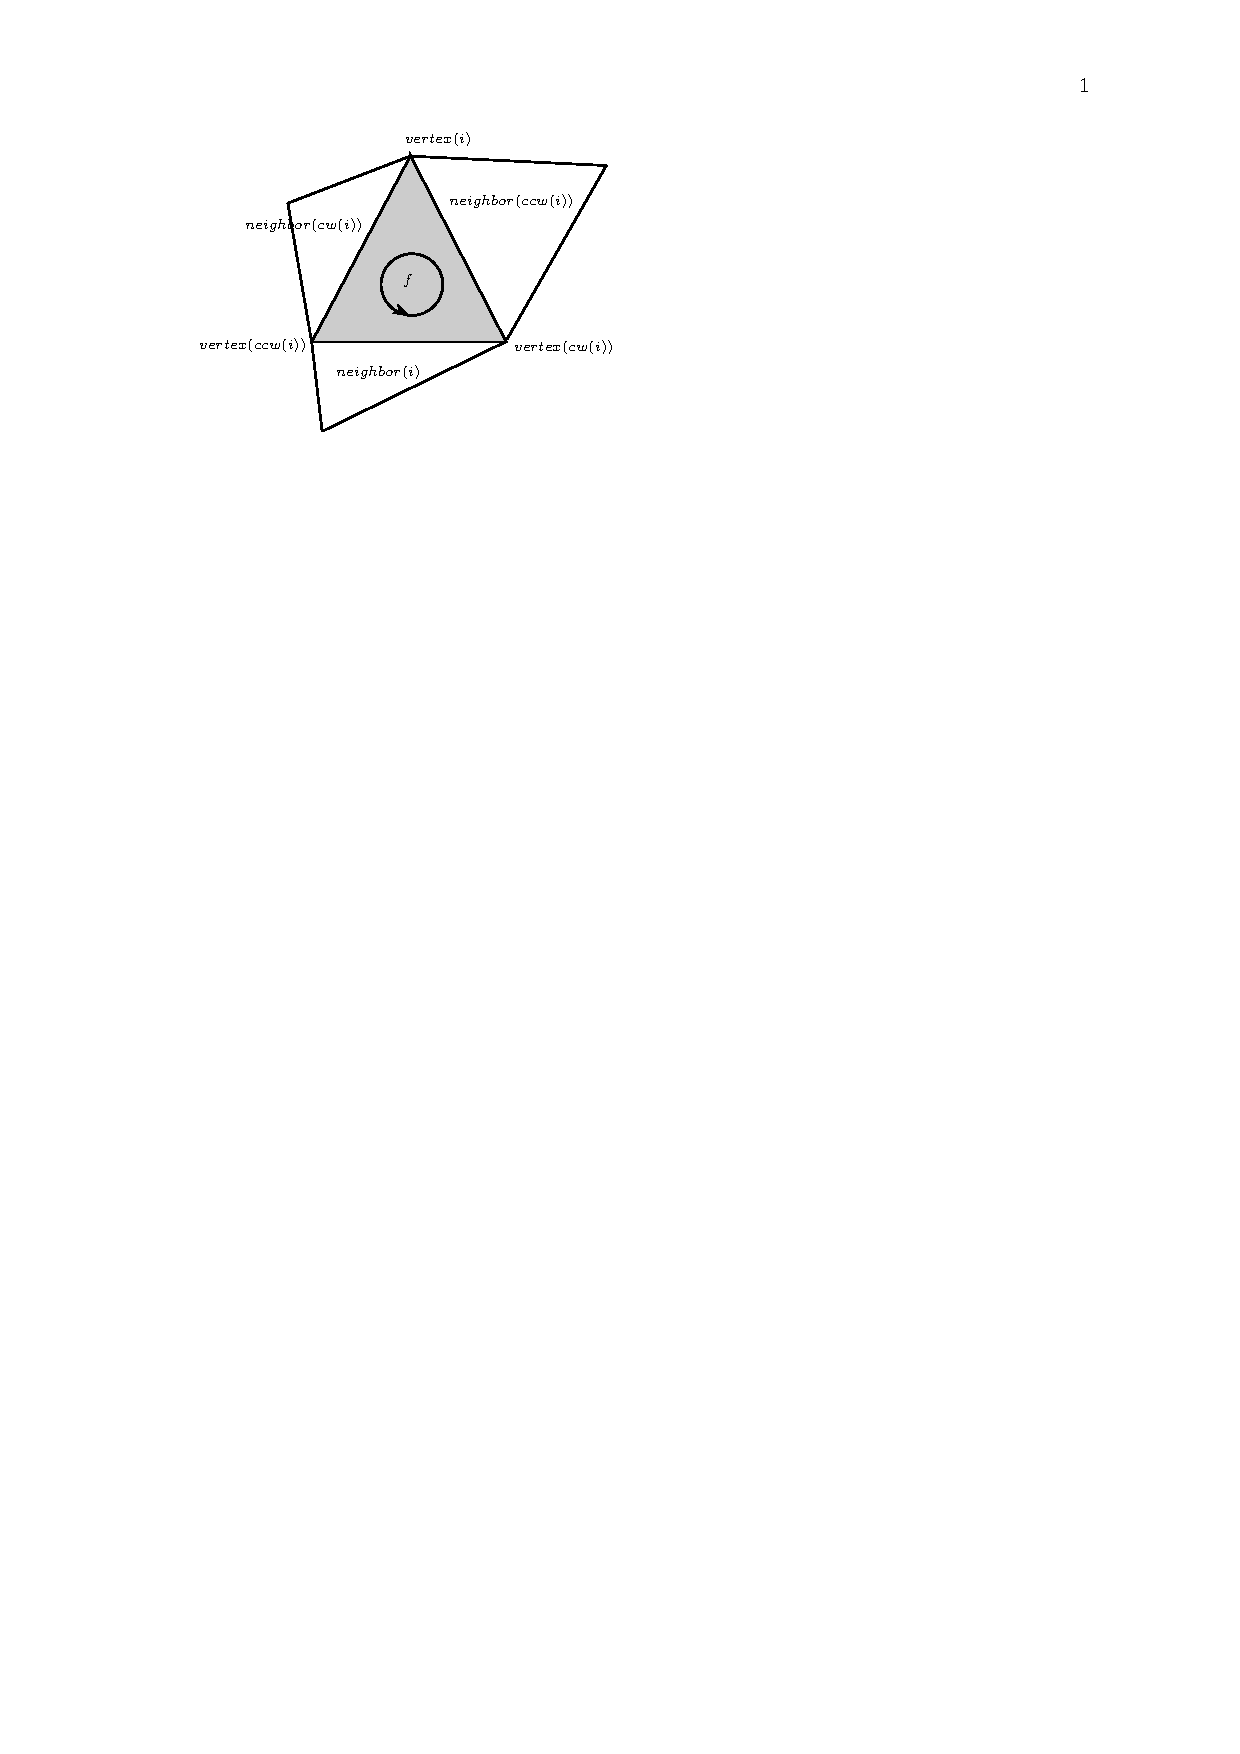
\includegraphics{Triangulation_2/neighbors}
    \end{center}
\end{ccTexOnly} 
    \caption{Vertices and neighbors.
    \label{Triangulation_ref_Fig_neighbors_bis}}
  \begin{ccHtmlOnly}
<CENTER>
<img border=0 src="./neighbors.gif" align=middle alt="Neighbors">
</CENTER>
\end{ccHtmlOnly} 
\end{figure}

\ccInclude{CGAL/Triangulation_2.h}



\ccCreation
\ccCreationVariable{a}  %% choose variable name

\ccConstructor{Triangulation_cw_ccw_2();}{default constructor.}

\ccOperations
\ccMethod{int ccw(const int i) const;}
{returns the index of the  neighbor or vertex that is  next to 
the neighbor or vertex with index \ccc{i}
in counterclockwise order around a face.}
\ccGlue
\ccMethod{int cw(const int i) const;}
{returns the index of the  neighbor or vertex that is  next to 
the neighbor or vertex with index \ccc{i}
in counterclockwise order around a face.}

\ccSeeAlso
\ccc{CGAL::Triangulation_2<Traits,Tds>} \\
\ccc{CGAL::TriangulationDSFace_2} \\

\end{ccRefClass}

% +------------------------------------------------------------------------+
%%RefPage: end of main body, begin of footer
% EOF
% +------------------------------------------------------------------------+


% +------------------------------------------------------------------------+
% | Reference manual page: Triangulation_data_structure_2.tex
% +------------------------------------------------------------------------+
% | 18.04.2002   Mariette Yvinec
% | Package: Triangulation_2
% | 
\RCSdef{\RCSTriangulationdatastructureRev}{$Revision$}
\RCSdefDate{\RCSTriangulationdatastructureDate}{$Date$}
% |
%%RefPage: end of header, begin of main body
% +------------------------------------------------------------------------+


\begin{ccRefClass}{Triangulation_data_structure_2<Vb,Fb>}  %% add template arg's if necessary

%% \ccHtmlCrossLink{}     %% add further rules for cross referencing links
%% \ccHtmlIndexC[class]{} %% add further index entries
\ccCreationVariable{tds}
\ccDefinition
  
The class \ccRefName\ is a  model
for the \ccc{TriangulationDataStructure_2} concept.
It can be used to represent an orientable 2D triangulation
embedded in a space of any dimension.

\ccInclude{CGAL/Triangulation_data_structure_2.h}

\ccIsModel
\ccc{TriangulationDataStructure_2}




\end{ccRefClass}

% +------------------------------------------------------------------------+
%%RefPage: end of main body, begin of footer
% EOF
% +------------------------------------------------------------------------+


\input{Triangulation_data_structure_2::Face.tex}
\input{Triangulation_data_structure_2::Vertex.tex}
% +------------------------------------------------------------------------+
% | Reference manual page: Triangulation_data_structure_using_list_2.tex
% +------------------------------------------------------------------------+
% | 07.04.2000   Author
% | Package: Package
% | 
\RCSdef{\RCSTriangulationdatastructureusinglistRev}{$Revision$}
\RCSdefDate{\RCSTriangulationdatastructureusinglistDate}{$Date$}
% |
%%RefPage: end of header, begin of main body
% +------------------------------------------------------------------------+


\begin{ccRefClass}{Triangulation_data_structure_using_list_2<Vb,Fb>}  %% add template arg's if necessary

%% \ccHtmlCrossLink{}     %% add further rules for cross referencing links
%% \ccHtmlIndexC[class]{} %% add further index entries
\ccCreationVariable{tds}
\ccDefinition
  
The class \ccRefName\ can be used as model
for the \ccc{TriangulationDataStructure_2} concept
 for any
orientable triangulation. It uses a \stl list to store the
full dimensional faces of the triangulation.


\ccInclude{Triangulation_data_structure_using_list_2.h}

\ccIsModel

\ccc{TriangulationDataStructure_2}



\end{ccRefClass}

% +------------------------------------------------------------------------+
%%RefPage: end of main body, begin of footer
% EOF
% +------------------------------------------------------------------------+


% +------------------------------------------------------------------------+
% | Reference manual page: Triangulation_default_data_structure_2.tex
% +------------------------------------------------------------------------+
% | 07.04.2000   Author
% | Package: Package
% | 
\RCSdef{\RCSTriangulationdefaultdatastructureRev}{$Revision$}
\RCSdefDate{\RCSTriangulationdefaultdatastructureDate}{$Date$}
% |
%%RefPage: end of header, begin of main body
% +------------------------------------------------------------------------+


\begin{ccRefClass}{Triangulation_default_data_structure_2<Traits,Vb,Fb>} 
 %% add template arg's if necessary

%% \ccHtmlCrossLink{}     %% add further rules for cross referencing links
%% \ccHtmlIndexC[class]{} %% add further index entries
\ccCreationVariable{tds}
\ccDefinition
  
The class \ccRefName\ is the default model for the concept
\ccc{TriangulationDataStructure_2}.
The class \ccRefName 
is highly economic with respect to memory space but its use is
restricted
to planar embedded triangulation.

As required this class has two template parameters \ccc{Vb} anf \ccc{Fb}
which have 
to be models for respectively the
\ccc{TriangulationVertexBase_2} and 
the \ccc{TriangulationFaceBase_2} concepts.

In addition, the class \ccClassTemplateName\ has a first template parameter
which is a geometric traits class. This may be surprising because
the triangulation data structure is supposed to deal only with the combinatorial
aspect of the triangulation and not with any geometric embedding
The reason for that is the following.
The class \ccRefName\ does not use any additional data structure
such as a list or a vector to act as a container for faces and vertices.
The iterators which allows to visit all faces and vertices of the
triangulation
data structure
is implemented using  an implicit tree structure over the faces
as described by
 de Berg, van Oostrum, and Overmars, 
in Proc.\ 12th Annual Symp.\ on Comput.\ Geom.,
1996, pages C5--C6. This tree structure is  based on the planar
geometric embedding
the triangulation. Each face 
 can find its parent 
and its children using only simple comparisons on the
coordinates of the points embedding its vertices.
Thus the tree structure may remain implicit 
and does not require any additional memory. 

The requirements concerning the geometric traits \ccc{Traits} of
\ccc{Triangulation_default_data_structure_2}
 are very light and form a subset of the concept
\ccc{TriangulationTraits_2}.
This class is required  to provide a type \ccc{Point}
and the coordinate comparison functions \ccc{compare_x(Point p0, Point p1)} and
\ccc{compare_y(Point p0, Point p1)}. The point type
defined by the geometric traits class of the triangulation data structure
has to be the same 
as the point type defined by the geometric traits of the triangulation.
This is achieved if the same model is used for both traits classes
which is recommended but not compulsory.


\ccInclude{Triangulation_default_data_structure_2.h}

\ccIsModel

\ccc{TriangulationDataStructure_2}


\ccSeeAlso

\ccc{TriangulationDataStructure_2},
\ccc{CGAL::Triangulation_data_structure_using_list_2<Vb,Fb>}.


\end{ccRefClass}

% +------------------------------------------------------------------------+
%%RefPage: end of main body, begin of footer
% EOF
% +------------------------------------------------------------------------+


% +------------------------------------------------------------------------+
% | Reference manual page: Triangulation_euclidean_traits_2.tex
% +------------------------------------------------------------------------+
% | 06.04.2000   Author
% | Package: Package
% | 
\RCSdef{\RCSTriangulationeuclideantraitsRev}{$Revision$}
\RCSdefDate{\RCSTriangulationeuclideantraitsDate}{$Date$}
% |
%%RefPage: end of header, begin of main body
% +------------------------------------------------------------------------+


\begin{ccRefClass}{Triangulation_euclidean_traits_2<R>}  %% add template arg's if necessary

%% \ccHtmlCrossLink{}     %% add further rules for cross referencing links
%% \ccHtmlIndexC[class]{} %% add further index entries
\ccCreationVariable{traits}
\ccDefinition
  
The class \ccRefName\ is a model for the \ccc{Triangulation_traits_2}
and \ccc{Delaunay_triangulation_traits_2} 
concepts. It uses types defined in \cgal\ kernel
as geometric primitives types.

\ccInclude{Triangulation_euclidean_traits_2.h}

\ccIsModel 

\ccc{TriangulationTraits_2} \\
\ccc{DelaunayTriangulationTraits_2}

\ccTypes
\ccThree{typedef Triangle_2<R>}{Triangle_2}{}
\ccTypedef{typedef CGAL::Point_2<R>  Point_2;}{}
\ccGlue
\ccTypedef{typedef CGAL::Segment_2<R>   Segment_2;}{}
\ccGlue
\ccTypedef{typedef CGAL::Triangle_2<R>   Triangle_2;}{}
\ccGlue
\ccTypedef{typedef CGAL::Line_2<R> Line_2;}{}
\ccGlue
\ccTypedef{typedef CGAL::Direction_2<R> Direction_2;}{}
\ccGlue
\ccTypedef{typedef CGAL::Ray_2<R>  Ray_2;}{}

The following predicates and constructor types are provided

\ccNestedType{Construct_segment_2}
\ccGlue
\ccNestedType{Construct_triangle_2}
\ccGlue
\ccNestedType{Compare_x_2}{}
\ccGlue
\ccNestedType{Compare_y_2}{}
\ccGlue
\ccNestedType{Orientation_2}{}
\ccGlue
\ccNestedType{Side_of_oriented_circle_2}{}
\ccGlue
\ccNestedType{Compare_distance_2}
\ccGlue
\ccNestedType{Construct_circumcenter_2}{}
\ccGlue
\ccNestedType{Construct_bisector_2}{}
\ccGlue
\ccNestedType{Construct_ray_2}{}
\ccGlue
\ccNestedType{Construct_direction_of_line_2}{}

\ccHeading{Access to predicate objects}
The following access functions are provided

\ccMethod{Construct_segment_2 construct_segment_2_object();}
\ccGlue
\ccMethod{Construct_triangle_2 construct_triangle_2_object();}
\ccGlue
\ccMethod{Comparison_x_2 compare_x_2_object();}{}                               \ccGlue
\ccMethod{Comparison_y_2 compare_y_2_object();}{}
\ccGlue
\ccMethod{Orientation_2  orientation_2_object();}{}
\ccGlue
\ccMethod{Side_of_oriented_circle_2
          side_of_oriented_circle_2_object();}{}
\ccGlue
\ccMethod{Compare_distance_2 compare_distance_2_object();}{}
\ccGlue
\ccMethod{Construct_circumcenter_2 construct_circumcenter_2_object();}{}
\ccGlue
\ccMethod{Construct_bisector_2 construct_bisector_2_object();}{}
\ccGlue
\ccMethod{Construct_ray_2 construct_ray_2_object();}{}
\ccGlue
\ccMethod{Construct_direction_of_line_2 
          construct_direction_of_line_2_object();}{} 

\ccSeeAlso
\ccc{TriangulationTraits_2} \\
\ccc{DelaunayTriangulationTraits_2} \\
\ccc{CGAL::Triangulation_2<Traits,Tds>}\\
\ccc{CGAL::Delaunay_triangulation_2<Traits,Tds>} \\
\ccc{CGAL::Triangulation_euclidean_traits_xy_3<R>} \\

\ccExample
The following code creates a  valid triangulation traits class 
for a triangulation of 2D points in usual Euclidean space
and use it to define a triangulation class.

\begin{cprog}

typedef Cartesian<double> Rp;
typedef Triangulation_euclidean_traits_2<Rp> Traits;
typedef Triangulation_vertex_base_2<Traits> Vb;
typedef Triangulation_face_base_2<Traits> Fb;
typedef Triangulation_data_structure_using_list_2<Vb,Fb > Tds;
typedef Triangulation_2<Traits,Tds> Triangulation;

\end{cprog}


\end{ccRefClass}

% +------------------------------------------------------------------------+
%%RefPage: end of main body, begin of footer
% EOF
% +------------------------------------------------------------------------+


% +------------------------------------------------------------------------+
% | Reference manual page: Triangulation_euclidean_traits_xy_3.tex
% +------------------------------------------------------------------------+
% | 06.04.2000   Author
% | Package: Package
% | 
\RCSdef{\RCSTriangulationeuclideantraitsxyRev}{$Id$}
\RCSdefDate{\RCSTriangulationeuclideantraitsxyDate}{$Date$}
% |
%%RefPage: end of header, begin of main body
% +------------------------------------------------------------------------+


\begin{ccRefClass}{Triangulation_euclidean_traits_xy_3<K>}  %% add template arg's if necessary

The functionality of this class has been generalized to other packages than 2D triangulations.
The more general class \ccc{Projection_traits_xy_3} can be found in the 2D and 3D Linear Geometric Kernel.

\begin{ccDeprecated}

%% \ccHtmlCrossLink{}     %% add further rules for cross referencing links
%% \ccHtmlIndexC[class]{} %% add further index entries
\ccCreationVariable{traits}
\ccDefinition
  
The class \ccRefName\ is a geometric traits class which allows to
triangulate
a terrain. This traits class is designed to build 
a two dimensional triangulation  embedded in 3D space,
i.e. a triangulated surface, such that 
its
on the $xy$ plane  is a Delaunay triangulation.
This is a usual construction for GIS terrains.
Instead of really projecting the 3D points and
maintaining a mapping between each point and its projection
 (which costs space and is error prone)
the class \ccRefName\  supplies geometric predicates that ignore the
\ccc{z}-coordinate of the points.

The class is a model of the concept \ccc{DelaunayTriangulationTraits_2} 
except that it does not provide the type and constructors
required to build the dual Voronoi diagram. The class is also a model
of the concept \ccc{ConstrainedTriangulationTraits_2}.

\ccParameters
The template parameter \ccc{K}  has to
be instantiated by a model of the \ccc{Kernel} concept.
\ccRefName\ uses types 
and predicates defined in \ccc{K}.

\ccInclude{CGAL/Triangulation_euclidean_traits_xy_3.h}

\ccTypes
\ccTwo{typedef Triangle_3<K>}{}
\ccTypedef{typedef Point_3<K>   Point_2;}{}
\ccGlue
\ccTypedef{typedef Segment_3<K>   Segment_2;}{}
\ccGlue
\ccTypedef{typedef Triangle_3<K>   Triangle_2;}{}
\ccGlue
\ccTypedef{typedef Line_3<K>   Line_2;}{}

The following predicates and constructor types are provided

\ccNestedType{Construct_segment_2}
{A constructor object for
\ccc{Segment_2}. Provides~: \\
\ccc{Segment_2 operator()(Point_2 p,Point_2 q)}, \\ 
which constructs a  segment from two points.}
\ccGlue
\ccNestedType{Construct_triangle_2}{A constructor object for
\ccc{Triangle_2}. Provides~: \\
\ccc{Triangle_2 operator()(Point_2 p,Point_2 q,Point_2 r )}, \\
which constructs a triangle from three points.}
\ccGlue
\ccNestedType{Construct_line_2}{A constructor object for
\ccc{Line_2}. Provides~: \\
\ccc{Line_2 operator()(Point_2 p,Point_2 q)}, \\
which constructs a line from two points.}
\ccGlue
\ccNestedType{Compute_squared_distance_2}{A construction object.
Provides the operator~:\\
\ccc{RT operator()(Line_2 l, Point_2 p);}
which returns the squared distance between the projection of \ccc{p} 
and the projection of \ccc{l}.}
\ccGlue
\ccNestedType{Intersect_2}{A construction object.
Provides the operator~:\\
\ccc{Object_2 operator()(Segment_2 s1, Segment_2 s2);}
which returns the intersection of the projection of \ccc{s1}
and the projection of \ccc{s2} embedded in \ccc{3D}. If the intersection
is a segment, the \ccc{z}-coordinates of its extremities is \ccc{0}.
If the intersection is a point \ccc{p}, let \ccc{p1} and \ccc{p2} be the points on \ccc{s1}
and \ccc{s2} respectively, such that their projections are \ccc{p}. The point returned is the
middle of the segment \ccc{p1}\ccc{p2}.
\ccPrecond{The projection of \ccc{s1} and the projection of \ccc{s2} are non-degenerate 
\ccc{2D} segments.}
}
\ccGlue
\ccNestedType{Compare_x_2}{Predicate object. Provides
the operator~: \\
\ccc{Comparison_result operator()(Point_2 p, Point_2 q)} \\
which returns 
\ccc{SMALLER, EQUAL} or \ccc{ LARGER}
 according to the
$x$-ordering of points \ccc{p} and \ccc{q}.}
\ccGlue
\ccNestedType{Compare_y_2}{Predicate object. Provides
the operator~: \\ 
\ccc{Comparison_result operator()(Point_2 p, Point_2 q)}\\
which returns 
(\ccc{SMALLER, EQUAL} or \ccc{ LARGER})
according to the
$y$-ordering of points \ccc{p} and \ccc{q}.}
\ccGlue
\ccNestedType{Orientation_2}{Predicate object. Provides
the  operator~: \\
\ccc{Orientation operator()(Point_2 p, Point_2 q, Point_2 r)}\\
which returns
\ccc{LEFT_TURN}, \ccc{RIGHT_TURN} or \ccc{COLLINEAR}
 according to the position of the projection of $r$
with respect to the projection of the 
oriented line \ccc{pq}.}
\ccGlue
\ccNestedType{Side_of_oriented_circle_2}{Predicate object. 
Provides the operator~:
\ccc{Oriented_side operator()(Point_2 p, Point_2 q, Point_2 r, Point_2 s)}
which takes four points $p, q, r, s$ as arguments and returns
\ccc{ON_POSITIVE_SIDE}, \ccc{ON_NEGATIVE_SIDE} or, 
\ccc{ON_ORIENTED_BOUNDARY} according to the position of 
the projection of point\ccc{s}
with respect to the oriented circle through the projections of $p,q$
and $r$.}
\ccGlue
\ccNestedType{Compare_distance_2} {Predicate object. Provides
 the operator : \\
\ccc{Comparison_result operator()(Point_2 p, Point_2 q, Point_2 r)}
which returns \ccc{SMALLER}, \ccc{EQUAL} or \ccc{LARGER}
according to the distance between the projection of p and the projection of q being smaller, equal or larger
than the distance between the projection of p and the projection of r.}

\ccCreation
\ccCreationVariable{traits}  %% choose variable name

\ccThree{Triangulation_euclidean_traits_xy_3()}{traits=tr  }{}

\ccConstructor{Triangulation_euclidean_traits_xy_3();}{
default constructor.}
\ccGlue
\ccConstructor{Triangulation_euclidean_traits_xy_3(
                      Triangulation_euclidean_traits_xy_3 tr);}
{Copy constructor.}
\ccMethod{Triangulation_euclidean_traits_xy_3 operator=
              (Triangulation_euclidean_traits_xy_3  tr);}
{Assignment operator.}


\ccHeading{Access to predicate objects}
The following access functions are provided

\ccThree{Side_of_oriented_circle_2}{side_of_oriented_circle_2_object();}{}
\ccMethod{Construct_segment_2 construct_segment_2_object();}{}
\ccGlue
\ccMethod{Construct_triangle_2 construct_triangle_2_object();}{}
\ccGlue
\ccMethod{Construct_line_2 construct_line_2_object();}{}
\ccGlue
\ccMethod{Comparison_x_2 compare_x_2_object();}{}
\ccGlue
\ccMethod{Comparison_y_2 compare_y_2_object();}{}
\ccGlue
\ccMethod{Orientation_2  orientation_2_object();}{}
\ccGlue
\ccMethod{Side_of_oriented_circle_2
side_of_oriented_circle_2_object();}{}
\ccGlue
\ccMethod{Compare_distance_2
compare_distance_2_object();} {}
\ccGlue
\ccMethod{Intersect_2  intersect_2_object();}{}
\ccGlue
\ccMethod{Compute_squared_distance_2 compute_squared_distance_2_object();}

\ccSeeAlso
\ccc{TriangulationTraits_2} \\
\ccc{DelaunayTriangulationTraits_2} \\
\ccc{CGAL::Triangulation_2<Traits,Tds>}\\
\ccc{CGAL::Delaunay_triangulation_2<Traits,Tds>} 


\cgal\ provides also predefined geometric traits class
\ccc{Triangulation_euclidean_traits_yz_3<K>} and
\ccc{Triangulation_euclidean_traits_xz_3<K>} to
deal with projections on the
 \ccc{xz}- or  the \ccc{yz}-plane,
respectively.

\ccInclude{CGAL/Triangulation_euclidean_traits_xz_3.h}\\
\ccInclude{CGAL/Triangulation_euclidean_traits_yz_3.h}

\end{ccDeprecated}
\end{ccRefClass}

% +------------------------------------------------------------------------+
%%RefPage: end of main body, begin of footer
% EOF
% +------------------------------------------------------------------------+


\input{Triangulation_face_base.tex}
% +------------------------------------------------------------------------+
% | Reference manual page: Triangulation_face_base_2.tex
% +------------------------------------------------------------------------+
% | 11.04.2000   Author
% | Package: Package
% | 
\RCSdef{\RCSTriangulationfacebaseRev}{$Revision$}
\RCSdefDate{\RCSTriangulationfacebaseDate}{$Date$}
% |
%%RefPage: end of header, begin of main body
% +------------------------------------------------------------------------+


\begin{ccRefClass}{Triangulation_face_base_2<Traits>}  %% add template arg's if necessary

%% \ccHtmlCrossLink{}     %% add further rules for cross referencing links
%% \ccHtmlIndexC[class]{} %% add further index entries
\ccCreationVariable{fb}
\ccDefinition
  
The class \ccRefName\ is the default  model for the concept
\ccc{TriangulationFaceBase_2}.
It is  templated by a geometric traits class.
Using for this traits class, the geometric traits class used for the triangulation class
is strongly recommended. 

These default base class can be used directly or can serve as a base to derive
other base classes with some additional attribute (a color for example)
tuned for a specific application.

\ccInclude{Triangulation_face_base_2.h}

\ccIsModel
\ccc{TriangulationFaceBase_2}

\ccSeeAlso
\ccc{TriangulationFaceBase_2}

\ccIndexHintAsSubitem[C]{Triangulation_2}{customizing faces or 
vertices}
\ccIndexHintAsSubitem[C]{Triangulation_face_base_2}{customizing}

\ccExample
The following example derives a new \ccc{Face_base} class from the default
one and add a color to the faces of the triangulation. 
The face of the triangulation data structure
and the face of the triangulation will inherit the new data member 
and its functionality.
Any kind of additional fonctionality can thus be added to faces or vertices of a triangulation 
as long as this functionality  does not involve additional pointers to vertices or faces
(because the base classes use only void* pointer and have no knowledge
of the vertex or face types.).


\ccIncludeExampleCode{Triangulation_2/colored_face.C}



\end{ccRefClass}

% +------------------------------------------------------------------------+
%%RefPage: end of main body, begin of footer
% EOF
% +------------------------------------------------------------------------+


% +------------------------------------------------------------------------+
% | Reference manual page: Triangulation_traits_2.tex
% +------------------------------------------------------------------------+
% | 06.04.2000   Author
% | Package: Package
% | 
\RCSdef{\RCSTriangulationtraitsRev}{$Revision$}
\RCSdefDate{\RCSTriangulationtraitsDate}{$Date$}
% |
%%RefPage: end of header, begin of main body
% +------------------------------------------------------------------------+


\begin{ccRefConcept}{Triangulation_traits_2}

%% \ccHtmlCrossLink{}     %% add further rules for cross referencing links
%% \ccHtmlIndexC[concept]{} %% add further index entries

\ccDefinition
  
The concept \ccRefName\ describes 
 the set of requirements to be
fulfilled
by any class used to instantiate the first template parameter of the class 
\ccc{Triangulation_2<Traits,Tds>}.
This concept provides the types of the geometric primitives used in the
triangulation and the required predicates on those primitives.

\ccTypes
\ccNestedType{Point}{The  type must provide
a copy constructor and assignment operator.}
\ccGlue
\ccNestedType{Segment}{The  type must provide a constructor that takes
two points as argument.}
\ccGlue
\ccNestedType{Triangle}{The type must provide a constructor that takes
three points as argument.}



\ccCreation
\ccCreationVariable{traits}  %% choose variable name
Only a default constructor and an assignement operator are required. 
Note that further constructors
can be provided. 

\ccConstructor{Triangulation_traits_2();}{default constructor.}
\ccGlue
\ccMethod{Triangulation_traits operator=(Triangulation_traits gtr);}
{Assignment operator.}

\ccHeading{Predicates}
\ccThree{Comparison_result}{gt.compare_x(Point p0, Point p1)x}{}
\ccMethod{Comparison_result compare_x(Point p0,
                                           Point p1);}
{Compares the \ccc{x}-coordinates.}
\ccGlue
\ccMethod{Comparison_result compare_y(Point p0,
                                           Point p1);}
{Compares the \ccc{y}-coordinates.}
\ccGlue
\ccMethod{bool compare(const Point& p0,
                       const Point& p1);}
{True if \ccc{compare_x(p0,p1)} and \ccc{compare_y(p0,p1)}
return \ccc{EQUAL}.}
\ccGlue
\ccMethod{Orientation orientation(const Point& p0,
                                       const Point& p1,
                                       const Point& p2);}
{Orientation test. }
\ccGlue
\ccMethod{Oriented_side side_of_oriented_circle(const Point &p,
					const Point &q,
					const Point &r,
					const Point &s) const;}
{Returns the oriented side of the query point \ccc{s}
with respect to the oriented circle going through \ccc{p,q,r}
in that order. This predicates is required
only if the function 
\ccc{ oriented_side(const Face_handle& f, const Point &p)}
is explicitely called by the user.}

\ccHeading{Construction}
\ccMethod{Point circumcenter(const Point &p, const Point &q, const Point &r) const; }
{Returns the center of the circle through \ccc{(p,q,r)}
This method is required only if the function
\ccc{circumcenter(Face_handle  f)} is called by the user.}



\ccHasModels
\ccc{Triangulation_euclidean_traits_2<R>}
\ccc{Triangulation_euclidean_traits_xy_3<R>}
\ccc{Triangulation_euclidean_traits_yz_3<R>}
\ccc{Triangulation_euclidean_traits_zx_3<R>}

\ccSeeAlso
\ccc{Triangulation_2<Traits,Tds>}



\end{ccRefConcept}

% +------------------------------------------------------------------------+
%%RefPage: end of main body, begin of footer
% EOF
% +------------------------------------------------------------------------+


\input{Triangulation_vertex_base.tex}
% +------------------------------------------------------------------------+
% | Reference manual page: Triangulation_vertex_base_2.tex
% +------------------------------------------------------------------------+
% | 11.04.2000   Author
% | Package: Package
% | 
\RCSdef{\RCSTriangulationvertexbaseRev}{$Id$}
\RCSdefDate{\RCSTriangulationvertexbaseDate}{$Date$}
% |
%%RefPage: end of header, begin of main body
% +------------------------------------------------------------------------+


\begin{ccRefClass}{Triangulation_vertex_base_2<Traits,Vb>}  
%% add template arg's if necessary

%% \ccHtmlCrossLink{}     %% add further rules for cross referencing links
%% \ccHtmlIndexC[class]{} %% add further index entries

\ccDefinition
  
The class \ccRefName\ is the default model for the concept
\ccc{TriangulationVertexBase_2}.

 \ccRefName\ can be simply plugged in the triangulation data
structure
of a triangulation, or used  as a base  class to derive
other base vertex classes tuned for specific applications.

\ccInclude{CGAL/Triangulation_vertex_base_2.h}

\ccParameters
\ccRefName\  is  templated by a geometric traits class which provide the type
\ccc{Point}. It is strongly recommended to instantiate this
traits class with the model used for the triangulation traits class.
This ensures that the point type defined by \ccRefName\
is the same as the point type defined by 
the triangulation.

The second template parameter of \ccRefName\ 
has to be a model of the concept \ccc{TriangulationDSVertexBase_2}
By default this parameter is
 instantiated by \ccc{CGAL::Triangulation_ds_vertex_base_2<>}.

\ccIsModel
\ccc{TriangulationVertexBase_2}

\ccInheritsFrom
\ccc{Vb}

\ccSeeAlso
\ccc{CGAL::Triangulation_ds_vertex_base_2<Tds>} \\
\ccc{CGAL::Triangulation_face_base_2<Traits,Fb>} \\
\ccc{CGAL::Regular_triangulation_vertex_base_2<Traits,Vb>} \\
\ccc{CGAL::Triangulation_vertex_base_with_info_2<Info,Traits,Vb>}

\end{ccRefClass}

% +------------------------------------------------------------------------+
%%RefPage: end of main body, begin of footer
% EOF
% +------------------------------------------------------------------------+


% +------------------------------------------------------------------------+
% | Reference manual page: Weighted_point.tex
% +------------------------------------------------------------------------+
% | 13.04.2000   Author
% | Package: Package
% | 
\RCSdef{\RCSWeightedpointRev}{$Id$}
\RCSdefDate{\RCSWeightedpointDate}{$Date$}
% |
%%RefPage: end of header, begin of main body
% +------------------------------------------------------------------------+


\begin{ccRefClass}{Weighted_point<Pt,Wt>}  %% add template arg's if necessary

%% \ccHtmlCrossLink{}     %% add further rules for cross referencing links
%% \ccHtmlIndexC[class]{} %% add further index entries

\ccDefinition
  
The class \ccRefName\ provides a type associating
a point type \ccc{Pt} with a weight type \ccc{Wt}.
It is used in the traits classes \ccc{Regular_triangulation_euclidean_traits_2}
and \ccc{Regular_triangulation_euclidean_traits_3}.

\ccInclude{CGAL/Weighted_point.h}

\ccInheritsFrom \ccc{Pt}

\ccTypes
\ccTypedef{Pt Point;}{The point type}
\ccGlue
\ccTypedef{Wt Weight;}{The weight type.}

\ccCreation
\ccCreationVariable{wp}  %% choose variable name
\ccConstructor{Weighted_point(Weighted_point wq)}{copy constructor.}
\ccGlue
\ccConstructor{Weighted_point(Point p=Point(), Weight w= Weight(0))}{}
\ccGlue
\ccConstructor{Weighted_point(FT x, FT y)}{Constructs the point from \ccc{x}
and \ccc{y} coordinates, with a weight of 0.  Requires that the ambient
dimension be 2.}
\ccGlue
\ccConstructor{Weighted_point(FT x, FT y, FT z)}{Constructs the point from
\ccc{x}, \ccc{y} and \ccc{z} coordinates, with a weight of 0.  Requires that
the ambient dimension be 3.}

\ccAccessFunctions
\ccMethod{Point point() const;}{}
\ccGlue
\ccMethod{ Weight weight() const;}{}


\ccSeeAlso
\ccc{CGAL::Regular_triangulation_euclidean_traits_2<Rep,Weight>}\\
\ccc{CGAL::Regular_triangulation_euclidean_traits_3<R,Weight>}.

\end{ccRefClass}


%% EOF
